\documentclass[8pt]{beamer}
\usetheme{MonMetropolis}


% Packages ----------------------------------------------------------------------------------------------------------------------


\usepackage[utf8]{inputenc}
\usepackage{booktabs}
\usepackage[scale = 2]{ccicons}
\usepackage{pgfplots}
\usepackage{xspace}
\usepackage{tikz, pgf}
\usepackage{bm}
\usepackage{flowchart}
\usepackage{mathtools}
\usepackage[font = {small, it}]{caption}
\usepackage[cyr]{aeguill}
\usepackage{amsmath}
\usepackage{amssymb}
\usepackage{array}
\usepackage[mathscr]{eucal}
\usepackage{eurosym}
\usepackage{subfigure}
\usepackage{colortbl, color}
\usepackage{icomma}
\usepackage[numbers]{natbib}
\usepackage{mathtools}
\usepackage{numprint}
\usepackage{booktabs}
\usepackage{mathrsfs}
\usepackage{fourier} 
\usepackage{makecell}
\usepackage{tabularx, ragged2e}
\usepackage{graphicx}
\usepackage{enumitem}
\usepackage[frenchb]{babel}
\usepackage{tcolorbox}
\usepackage{lipsum}
\usepackage{tabu}
\usepackage{array}
\usepackage{smartdiagram}
% \usepackage{algorithmic}
\usepackage{bbm}
\usepackage{xfrac}
\usepackage{adjustbox}
% \usepackage{algorithm}
% \usepackage{algorithm2e}
\usepackage{pifont}
\usepackage{bbold}
\usepackage[usenames, dvipsnames]{xcolor}
\usepackage[autostyle]{csquotes}
\usepackage[absolute, overlay]{textpos}
\usepackage[colorlinks = true, linkcolor = bluecite, urlcolor = bluecite]{hyperref}
\usepackage{textcomp}

\usetikzlibrary{calc}
\setbeamertemplate{footline}[frame number]


\usepackage{framed,color,verbatim}
\colorlet{shadecolor}{mgris!7}

\newenvironment{code}%
   {\snugshade\verbatim}%
   {\endverbatim\endsnugshade}



\definecolor{bluecite}{HTML}{0875b7}
\hypersetup{citecolor = bluecite}



% Autres commandes --------------------------------------------------------------------------------------------------------------

\usepgfplotslibrary{dateplot}
\usesmartdiagramlibrary{additions}
\usetikzlibrary{shapes, arrows, chains, arrows.meta, positioning, quotes, matrix, snakes, trees, shadows, calc, shapes.geometric, shapes.misc}
\newcommand\blt{\item[$\bullet$]}
\newcommand\fleche{\item[$\blacktriangleright$]}
\newcommand{\themename}{\textbf{\textsc{metropolis}}\xspace}
\newcommand{\defeq}{\vcentcolon=}
\renewcommand\theadalign{bc}
\renewcommand\theadfont{\bfseries}
\renewcommand\theadgape{\Gape[4pt]}
\renewcommand\cellgape{\Gape[4pt]}
\newcommand{\emphcol}[1]{\textcolor{morange}{#1}}
\newcommand{\argmin}[1]{\underset{#1}{\operatorname{arg}\,\operatorname{min}}\;}
\newcommand{\argmax}[1]{\underset{#1}{\operatorname{arg}\,\operatorname{max}}\;}
\newcolumntype{?}{!{\vrule width 1pt}}
\DeclareMathOperator*{\moyenne}{average}
\metroset{sectionpage = none}

\newcommand{\cmark}{\textcolor{green!80!black}{\ding{51}}}
\newcommand{\xmark}{\textcolor{red}{\ding{55}}}
\newcommand * \circled[1]{\tikz[baseline = (char.base)]{\node[shape = circle, draw, inner sep = 2pt, thick, fill = mgris, color = mgris, text = white, font = \bfseries, scale = 0.8] (char) {#1};}}

\definecolor{light_red}{HTML}{f6a4a4}
\newcommand{\motcle}[1]{\bm{\textcolor{mon_rouge}{{#1}}}}
\newenvironment{variableblock}[3]{%
  \setbeamercolor{block body}{#2}
  \setbeamercolor{block title}{#3}
  \begin{block}{#1}}{\end{block}}
  
\newcommand{\motclef}[1]{\textcolor{mon_rouge}{{#1}}}
  
 
\AtBeginSection[]{
  \begin{frame}
  \centering	
  \Huge 
  \textcolor{mbleufonce}{\insertsection}
  \end{frame}
}

\newcounter{exemple}
\newenvironment{exemple}[1][]{
    \refstepcounter{exemple}
    \begin{exampleblock}{Exemple~\theexemple}}
    {\end{exampleblock}}

\newcounter{propo}
\newenvironment{propo}[1][]{
    \refstepcounter{propo}
    \begin{block}{Proposition~\thepropo}}
    {\end{block}}

  
% Page-titre --------------------------------------------------------------------------------------------------------------------

\title{\huge Analyse en composantes principales\\{\normalfont\Large Analyse de données en actuariat (ACT-6100)}}
\date{\large Automne 2021}  
\author{\Large Francis Duval}
\institute{\normalsize Université du Québec à Montréal}
\titlegraphic{\hspace{-0.45cm}
\includegraphics[width = 3.2cm]{logoUQAM.pdf}}


% Document principal ------------------------------------------------------------------------------------------------------------

\begin{document}
\maketitle

\begin{frame}{Contenu}
 	\setbeamertemplate{section in toc}[sections numbered]
 	\setbeamertemplate{subsection in toc}{\leavevmode\leftskip=2em\rlap{\hskip-2em$\quad$\inserttocsectionnumber.\inserttocsubsectionnumber}$\quad$\inserttocsubsection\par}
  	\tableofcontents[]
\end{frame}

% ------------------------------------------------------------------------------------------------------------------------------

\section{Introduction}

% ------------------------------------------------------------------------------------------------------------------------------

\begin{frame}{Lapin de Standford}

\begin{figure}
    \centering
    \begin{subfigure}{\textwidth}
        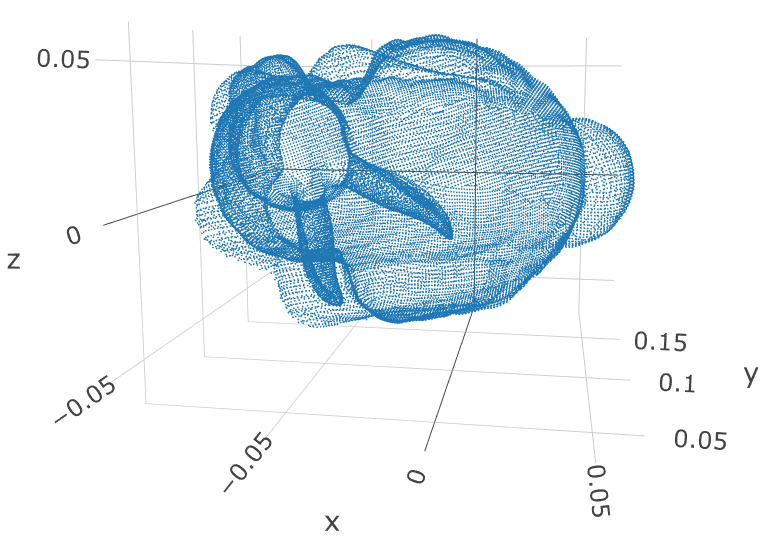
\includegraphics[scale = 0.248]{lapin_bas.png}
    \end{subfigure}
    \begin{subfigure}{\textwidth}
        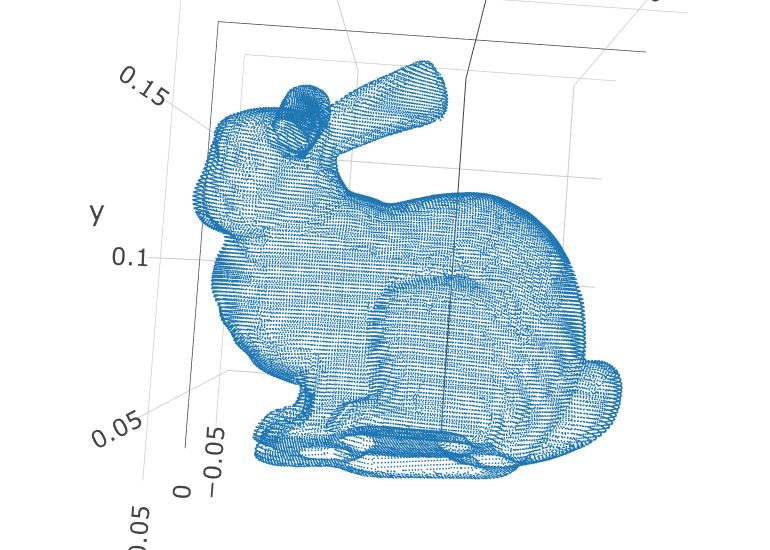
\includegraphics[scale = 0.248]{lapin_cote.png}
    \end{subfigure}
    \begin{subfigure}{\textwidth}
        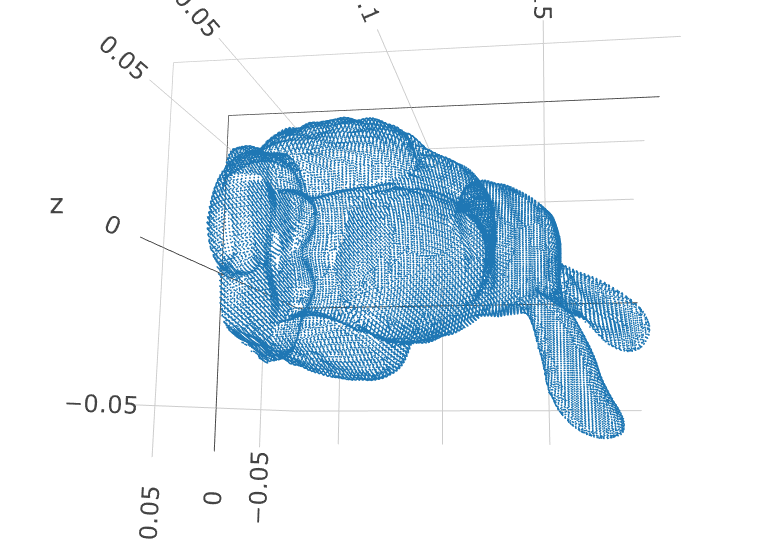
\includegraphics[scale = 0.248]{lapin_derriere.png}
    \end{subfigure}

    \medskip

    \begin{subfigure}{\textwidth}
        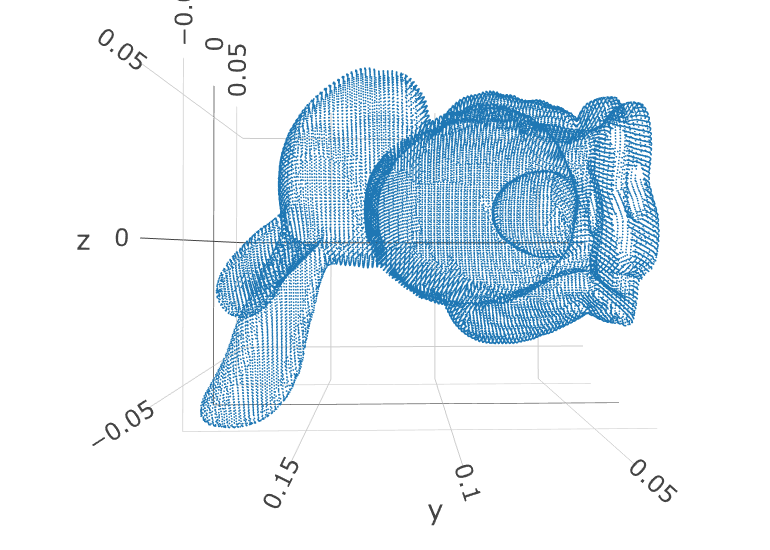
\includegraphics[scale = 0.248]{lapin_devant.png}
    \end{subfigure}
    \begin{subfigure}{\textwidth}
        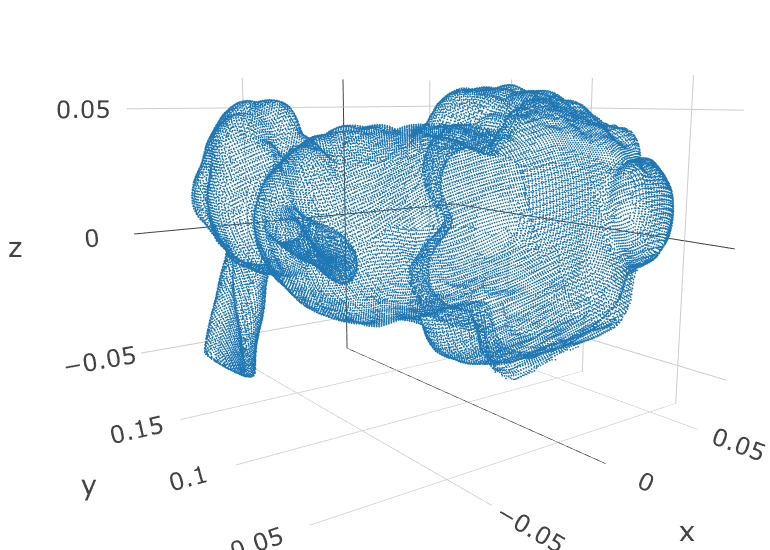
\includegraphics[scale = 0.248]{lapin_diagonale.png}
    \end{subfigure}
    \begin{subfigure}{\textwidth}
        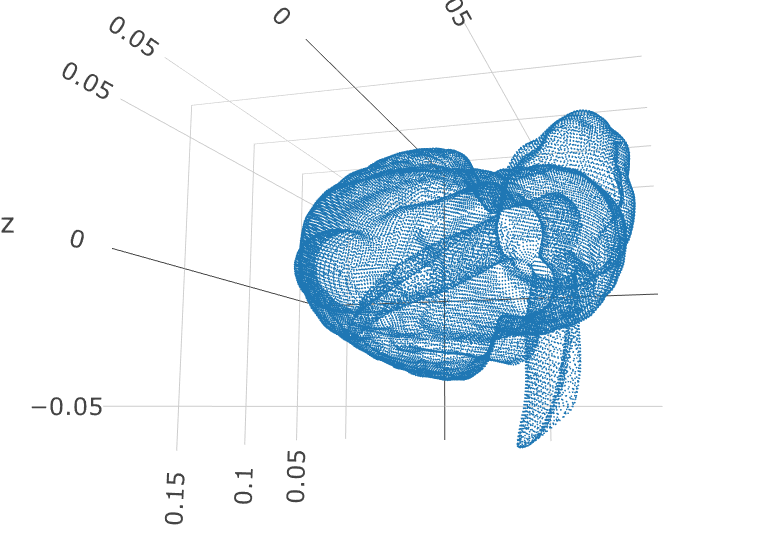
\includegraphics[scale = 0.248]{lapin_haut.png}
    \end{subfigure}
\end{figure}

\textbf{Quelle est la meilleure projection?}

\end{frame}

% ------------------------------------------------------------------------------------------------------------------------------

\begin{frame}[fragile]{Lapin de Stanford}
    
\textbf{Projection en 2 dimensions du jeu de données grâce à l'ACP}


\begin{code}
> library(tidyverse)
> library(onion)
> theme_set(theme_bw())
> 
> acp <- prcomp(bunny)
> ggplot(as_tibble(acp[["x"]]), aes(x = PC1, y = PC2)) +
+   geom_point(size = 0.1)
\end{code}

\begin{figure}
    \centering
    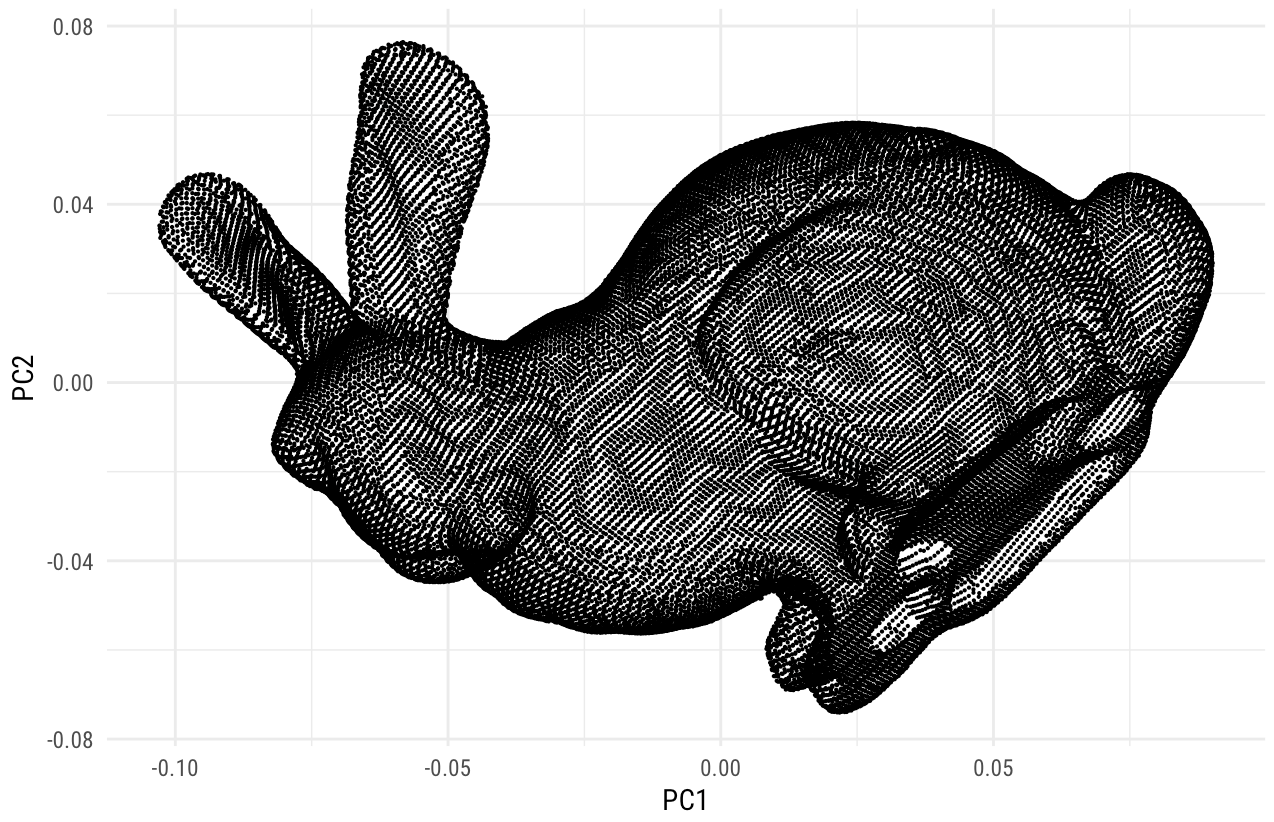
\includegraphics[scale = 0.3]{lapin_standford_acp.png}
\end{figure}

\end{frame}

% ------------------------------------------------------------------------------------------------------------------------------

\begin{frame}{ACP en 2 dimensions}

\begin{figure}
    \centering
    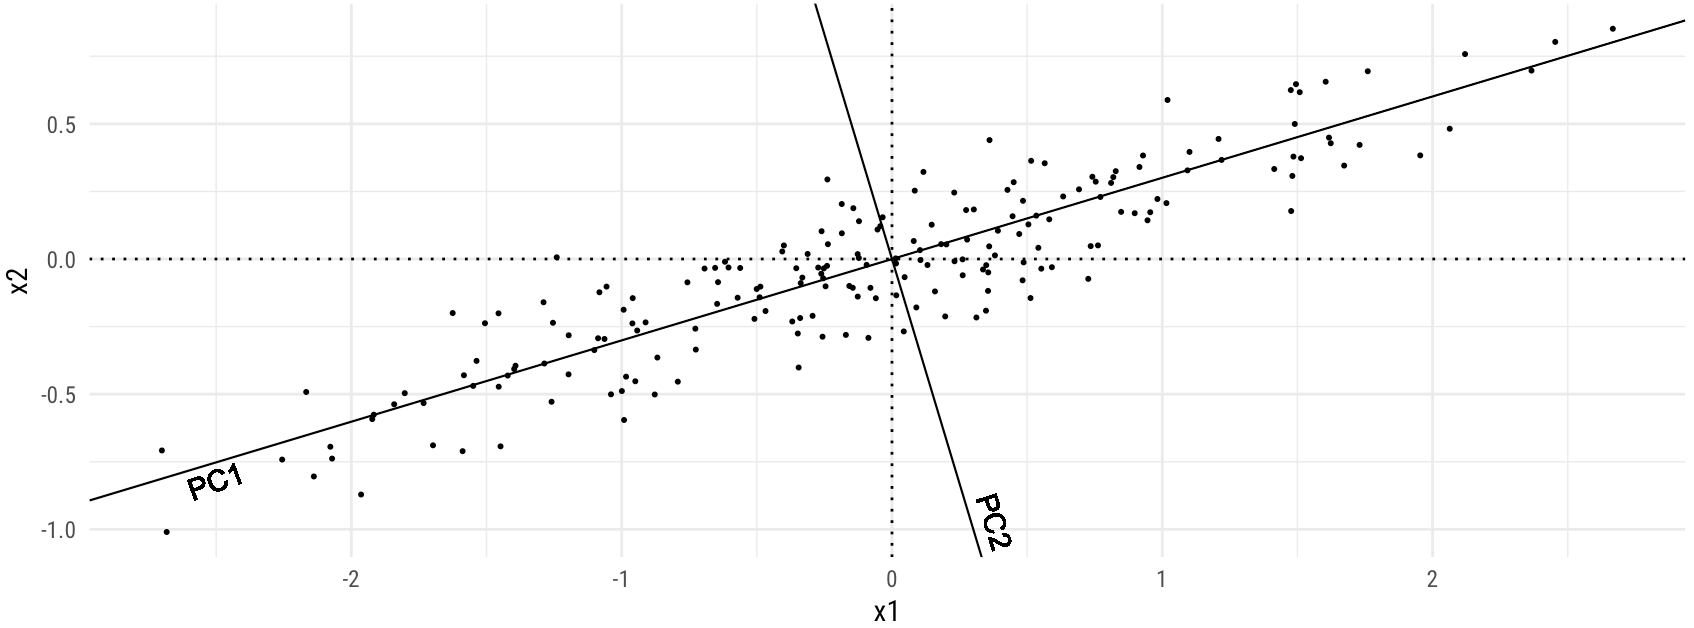
\includegraphics[scale = 0.35]{pca_2d_2.png}
\end{figure}

\begin{itemize}
    \fleche L'ACP va d'abord trouver le premier axe principal (PC1), c'est-à-dire la droite passant par $(0, 0)$ qui maximise la variance des points projetés orthogonalement sur celle-ci.
    \fleche Ensuite, l'ACP va trouver le deuxième axe principal (PC2), c'est-à-dire la droite passant par $(0, 0)$ qui maximise la variance des points projetés sur celle-ci \motcle{parmi tous les axes orthogonaux à l'axe PC1}.
    \begin{itemize}
        \item[-] Noter qu'ici, puisqu'on est en 2D, il n'y a qu'un seul axe orthogonal à la droite PC1 passant par $(0, 0)$. 
    \end{itemize}
\end{itemize}

\end{frame}

% ------------------------------------------------------------------------------------------------------------------------------

\begin{frame}[fragile]{Données}
    
\small
\begin{itemize}
    \fleche Le but est d'explorer un jeu de données \motcle{numérique}.
    \fleche Exemple: extrait de la base de données \href{https://statsandr.com/blog/data/Eurojobs.csv}{\textcolor{blue}{\underline{\texttt{eurojob}}}}, qui décrit les composantes de l'économie pour certains pays
    \begin{code}
> library(tidyverse)
> eurojob <- read_csv("https://statsandr.com/blog/data/Eurojobs.csv")
> x <- 
+   eurojob[1:6, 1:4] %>%
+   column_to_rownames("Country") %>% 
+   as.matrix()

> x
            Agr Min  Man
Belgium     3.3 0.9 27.6
Denmark     9.2 0.1 21.8
France     10.8 0.8 27.5
W. Germany  6.7 1.3 35.8
Ireland    23.2 1.0 20.7
Italy      15.9 0.6 27.6
    \end{code}
    \fleche Les lignes décrivent les \motcle{observations ou les individus} (les 6 pays) alors que les colonnes décrivent les \motcle{variables} (les 3 secteurs de l'économie: agriculture, minier et manufacturier).
    \fleche On veut savoir:
    \begin{itemize}
        \item[-] quelles observations sont similaires,
        \item[-] quelles variables sont liées.
    \end{itemize}
\end{itemize}

\end{frame}

% ------------------------------------------------------------------------------------------------------------------------------


\begin{frame}[fragile]{Matrices de distances et de corrélations}

On peut observer:

\begin{itemize}
    \fleche La matrice des \motcle{distances} entre individus:
    \begin{code}
> dist(x)
             Belgium   Denmark    France W. Germany   Ireland
Denmark     8.312039                                         
France      7.501333  5.961543                               
W. Germany  8.885944 14.272001  9.270922                     
Ireland    21.062526 14.071958 14.143550  22.368505          
Italy      12.603571  8.875810  5.104900  12.343824 10.052860
    \end{code}
    \fleche La matrice des \motcle{corrélations} entre variables:
    \begin{code}
> cor(x)
            Agr         Min        Man
Agr  1.00000000 -0.01026054 -0.5573922
Min -0.01026054  1.00000000  0.6117080
Man -0.55739225  0.61170803  1.0000000
    \end{code}
\end{itemize}

\end{frame}

% ------------------------------------------------------------------------------------------------------------------------------

\begin{frame}[fragile]{Visualisation des distances et corrélations}

\begin{itemize}
    \fleche L'ACP permet de visualiser sur un graphique les \motcle{distances entre individus} ainsi que les \motcle{corrélations entre variables}.
\end{itemize}


\begin{columns}[T]
    \begin{column}{0.48\textwidth}
        \begin{figure}
            \centering
            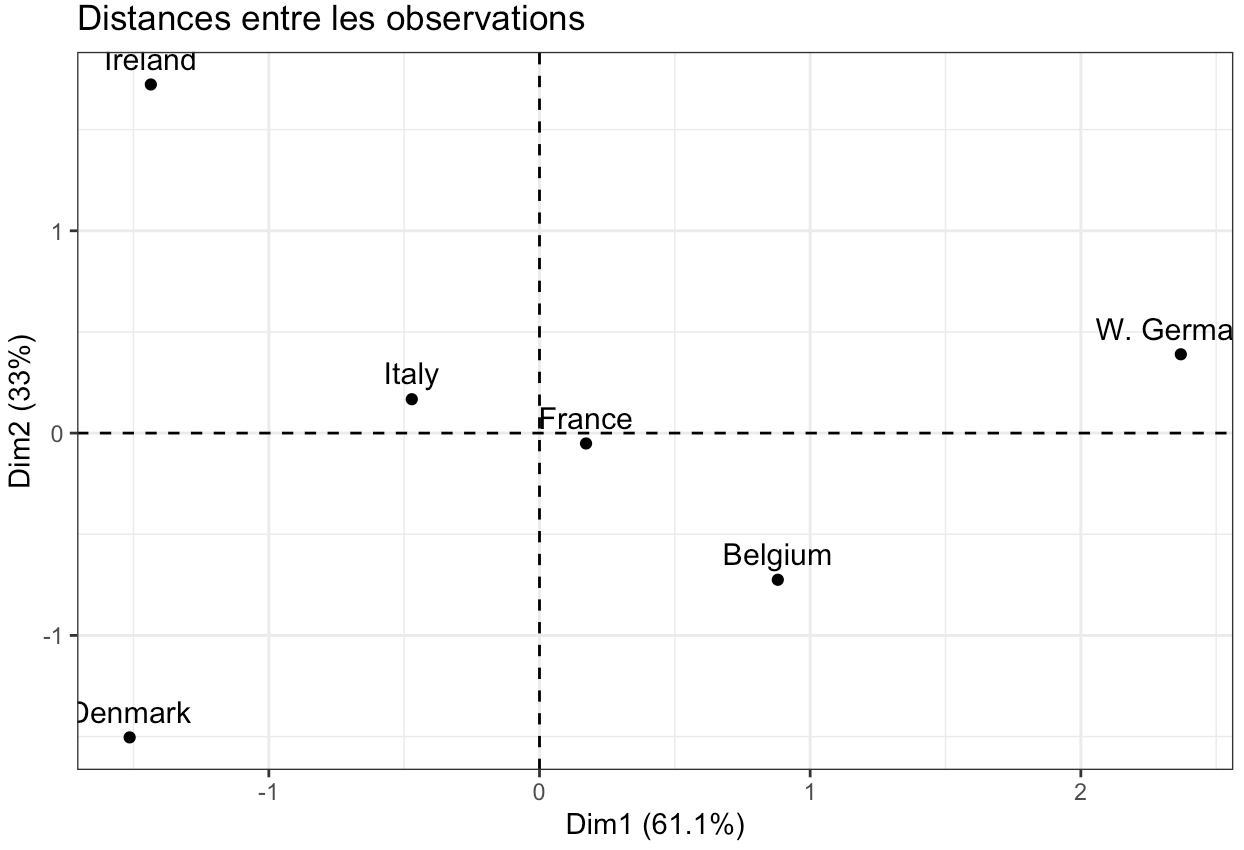
\includegraphics[scale = 0.27]{distances_observations.png}
        \end{figure}
    \end{column}
    \begin{column}{0.48\textwidth}
        \begin{figure}
            \centering
            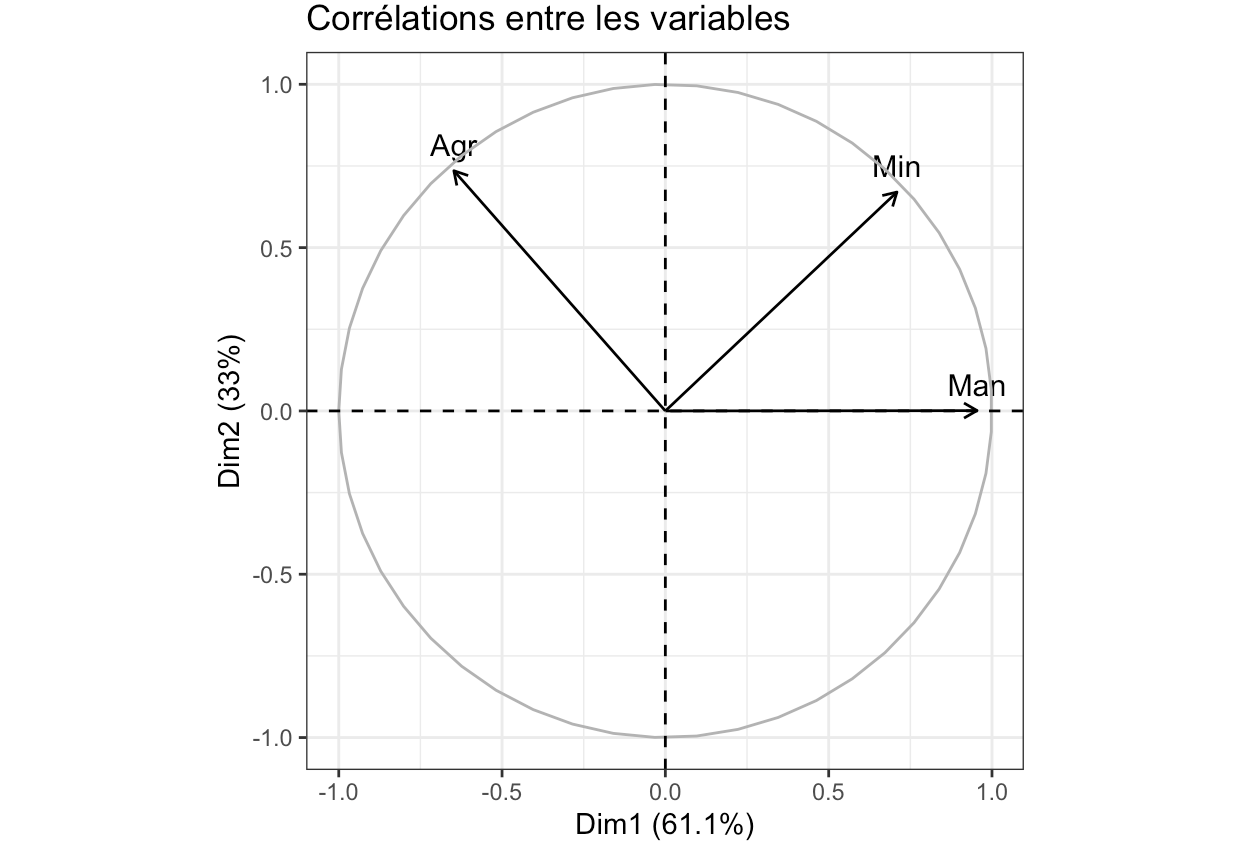
\includegraphics[scale = 0.27]{correlations_variables.png}
        \end{figure}
    \end{column}
\end{columns}


\end{frame}

% ------------------------------------------------------------------------------------------------------------------------------

\begin{frame}[fragile]{But de l'ACP}
\small
\begin{itemize}
    \fleche Construire de nouvelles variables numériques qui résument le mieux possible les variables originales afin de \motcle{réduire la dimension} du jeu de données.
    \begin{code}
> library(FactoMineR)

> # Jeu de données original
> x
            Agr Min  Man
Belgium     3.3 0.9 27.6
Denmark     9.2 0.1 21.8
France     10.8 0.8 27.5
W. Germany  6.7 1.3 35.8
Ireland    23.2 1.0 20.7
Italy      15.9 0.6 27.6

> # Nouvelles variables synthétiques
> acp <- PCA(x)
> acp$ind$coord
                Dim.1       Dim.2       Dim.3
Belgium     0.8804620 -0.72493205 -0.65397292
Denmark    -1.5141449 -1.50391377  0.06360123
France      0.1719596 -0.05132316  0.02039562
W. Germany  2.3694452  0.38961453  0.21632994
Ireland    -1.4359290  1.72305846 -0.33486793
Italy      -0.4717928  0.16749598  0.68851406
    \end{code}
\end{itemize}

\end{frame}


% ------------------------------------------------------------------------------------------------------------------------------

\begin{frame}{En résumé}
    
\small
\begin{itemize}
    \fleche L'analyse en composantes principales (ACP) est une méthode de \motcle{réduction de dimensions}.
    \begin{itemize}
        \item[-] Dans un jeu de données, le nombre de dimensions correspond au nombre de \motcle{variables}.
        \item[-] L'ACP permet donc de réduire le nombre de variables dans un jeu de données tout en \motcle{préservant un maximum d'information}.
        \item[-] On souhaite décrire la variablilité (l'inertie) présente dans un ensemble de variables initiales corrélées
        \begin{align*}
            X_1, \dots, X_k
        \end{align*}
        à l'aide d'un nouvel ensemble de variables non-corrélées
        \begin{align*}
            PC_1, \dots, PC_k,
        \end{align*}
        appelées \motcle{composantes principales}.
        \item[-] Chacune des nouvelles variables $PC_j, j = 1, \dots, k$, est une combinaison linéaire des variables initiales $X_j, j = 1, \dots, k$:
        \begin{align*}
            PC_j = a_{j1} X_1 + a_{j2} X_2 + \dots + a_{jk} X_k.
        \end{align*}
        \item[-] Pour réduire la dimensionnalité, l'ACP \motcle{projette} (de manière optimale) le nuage de points des observations dans $\mathbb{R}^k$ dans l'espace $\mathbb{R}^{k^*}$, où $k^* < k$.
        \item[-] « Préserver un maximum d'information » signifie qu'on veut que 2 points qui sont \motcle{proches dans l'espace $\mathbb{R}^k$} soient également \motcle{proches dans l'espace $\mathbb{R}^{k^*}$}. 
        \item[-] De la même manière, on veut que 2 points qui sont \motcle{éloignés dans l'espace $\mathbb{R}^k$} soient également \motcle{éloignés dans l'espace $\mathbb{R}^{k^*}$}.
    \end{itemize}
    \fleche C'est par le fait même un outil de \motcle{visualisation des données} puisqu'elle permet de visualiser des jeux de données en plus de 3 dimensions.
\end{itemize}

\end{frame}

% ------------------------------------------------------------------------------------------------------------------------------

\section{Concepts de base}

% ------------------------------------------------------------------------------------------------------------------------------

\subsection{Nuage des observations}

% ------------------------------------------------------------------------------------------------------------------------------

\begin{frame}{Notation}
    \begin{itemize}
        \fleche On considère une base de données numérique où $n$ observations sont décrites avec $p$ variables.
        \begin{table}
            \centering
            \begin{tabular}{c|ccccc|}
                & 1 & \cdots & $j$ & \cdots & $p$\\
                \midrule
                1 &  &  &  &  & \\
                \vdots &  &  & \vdots &  & \\
                $i$ &  & \cdots & $x_{ij}$ & \cdots & \\
                \vdots &  &  & \vdots &  & \\
                $n$ &  &  &  &  & \\
                \midrule
            \end{tabular}
        \end{table}
        \fleche Un peu de notation:
        \begin{itemize}
            \blt $\boldsymbol{X} = (x_{ij})_{n\times p}$ est la matrice des données, où $x_{ij}$ est la valeur de la $i^\text{e}$ observation pour la $j^\text{e}$ variable.
            \blt La $i^\text{e}$ ligne et la $j^\text{e}$ colonne de $\boldsymbol{X}$ sont notées respectivement
            \begin{align*}
                \boldsymbol{x}_i = \begin{pmatrix}x_{i1}\\\vdots \\ x_{ip}\end{pmatrix}\in \mathbb{R}^p \quad \text{et} \quad \boldsymbol{x}^j = \begin{pmatrix}x_{1j}\\\vdots \\ x_{nj}\end{pmatrix}\in \mathbb{R}^n.
            \end{align*}
        \end{itemize}

    \end{itemize}
\end{frame}


% -------------------------------------------------------------------------------------------------------------------
%-----------

\begin{frame}{Nuage des observations}
\small
\textbf{Exemple}: les 6 pays d'\texttt{eurojob} définissent un nuage de points de $n = 6$ points dans $\mathbb{R}^3$.
    
\begin{figure}
    \centering
    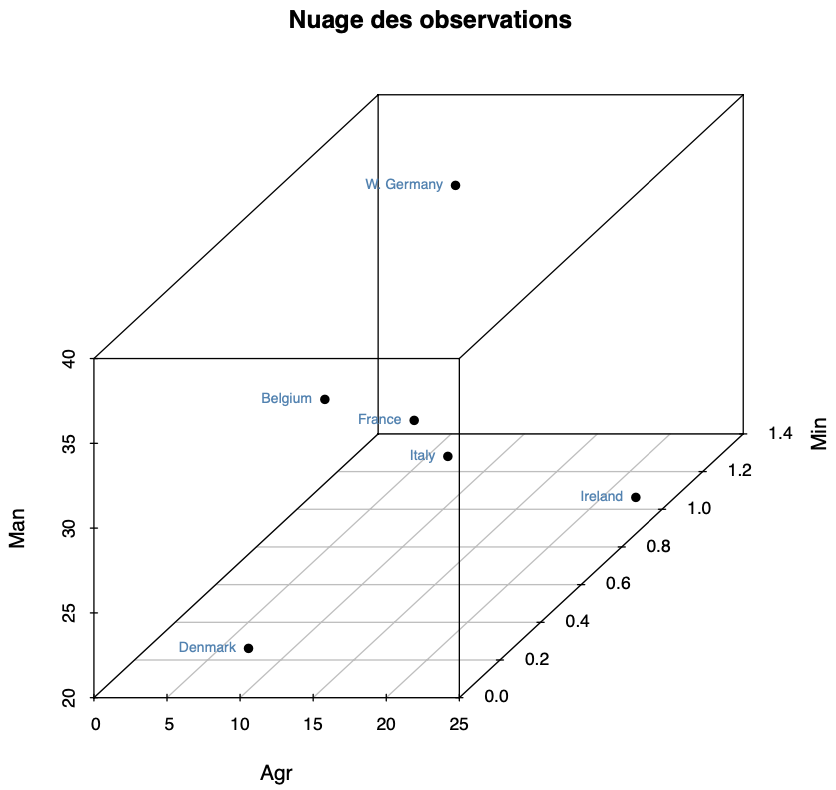
\includegraphics[scale = 0.37]{nuage_observations.png}
\end{figure}
    
\begin{itemize}
    \fleche Les $n$ lignes de $\boldsymbol{X}$, $\boldsymbol{x}_i$ pour $i = 1, \dots n$, définissent un nuage de points dans $\mathbb{R}^p$.
    \fleche Chaque observation $i$ est un \motcle{point $\boldsymbol{x}_i$ dans $\mathbb{R}^p$}.
    \fleche Un \motclef{poids $w_i$} est associé à chaque observation. Habituellement:
    \begin{itemize}
        \item[-] $w_i = \frac{1}{n}$ pour des observations tirées au hasard
        \item[-] $w_i \ne \frac{1}{n}$ pour des observations aggrégées, etc.
    \end{itemize}
    \fleche Pour réaliser une ACP, on a besoin du \motcle{nuage centré} ou du \motcle{nuage centré-réduit}.
\end{itemize}
    
\end{frame}

% ------------------------------------------------------------------------------------------------------------------------------

\begin{frame}{Nuage centré des observations}

\small
\begin{columns}[T]
    \begin{column}{0.48\textwidth}
        Matrice des données \motcle{originale} $\boldsymbol{X}$
        \begin{table}
            \centering
            \begin{tabular}{c|ccccc|}
                & 1 & \cdots & $j$ & \cdots & $p$\\
                \midrule
                1 &  &  &  &  & \\
                \vdots &  &  & \vdots &  & \\
                $i$ &  & \cdots & $x_{ij}$ & \cdots & \\
                \vdots &  &  & \vdots &  & \\
                $n$ &  &  &  &  & \\
                \midrule
                \midrule
                $\boldsymbol{\overline{x}}$ &  & \cdots & $\overline{x}^j$ & \cdots &
            \end{tabular}
        \end{table}
    \end{column}
    \begin{column}{0.48\textwidth}
        Matrice des données \motcle{centrée} $\boldsymbol{Y}$
        \begin{table}
            \centering
            \begin{tabular}{c|ccccc|}
                & 1 & \cdots & $j$ & \cdots & $p$\\
                \midrule
                1 &  &  &  &  & \\
                \vdots &  &  & \vdots &  & \\
                $i$ &  & \cdots & $y_{ij}$ & \cdots & \\
                \vdots &  &  & \vdots &  & \\
                $n$ &  &  &  &  & \\
                \midrule
                \midrule
                $\boldsymbol{\overline{y}}$ &  & \cdots & $0$ & \cdots &
            \end{tabular}
        \end{table}
    \end{column}
\end{columns}

Ici:
\begin{itemize}
    \fleche $\overline{x}^j$ est la moyenne empirique de la $j^\text{e}$ variable,
    \fleche \motclef{$y_{ij} = x_{ij} - \overline{x}^j$} est le terme générique de la matrice centrée des données $\boldsymbol{Y}$.
    \fleche Les colonnes de la \motcle{matrice centrée $\boldsymbol{Y}$} ont une moyenne de 0:
    \begin{align*}
        \boldsymbol{\overline{y}} = \frac{1}{n}\sum_{i = 1}^n y_{ij} = 0.
    \end{align*}
    \fleche Le nouveau centre de gravité du nuage est le point d’origine.
    \fleche Les distances entre les observations sont préservées, c'est-à-dire que
    \begin{align*}
        d_{\boldsymbol{M}}(\boldsymbol{x}_i, \boldsymbol{x}_j) = d_{\boldsymbol{M}}(\boldsymbol{y}_i, \boldsymbol{y}_j),
    \end{align*}
    où $d_{\boldsymbol{M}}(\cdot, \cdot)$ est une mesure de distance.
\end{itemize}

\end{frame}

% ------------------------------------------------------------------------------------------------------------------------------

\begin{frame}[fragile]{Nuage centré des observations}

\small
\textbf{Exemple:} jeu de données \texttt{eurojob}

\begin{code}
> # Centrer la matrice des données x
> y <- x
> for(j in 1:ncol(x)) {
+     y[ , j] <- x[ , j] - mean(x[ , j])
+ }
\end{code}

\begin{columns}[T]
    \begin{column}{0.45\textwidth}
        Matrice des données \motcle{originale} $\boldsymbol{X}$
        \begin{code}
> round(x, 4)
            Agr Min  Man
Belgium     3.3 0.9 27.6
Denmark     9.2 0.1 21.8
France     10.8 0.8 27.5
W. Germany  6.7 1.3 35.8
Ireland    23.2 1.0 20.7
Italy      15.9 0.6 27.6
        \end{code}
        Moyennes des colonnes de $\boldsymbol{X}$
        \begin{code}
> round(colMeans(x), 4)
    Agr     Min     Man 
11.5167  0.7833 26.8333
        \end{code}
    \end{column}
    \begin{column}{0.45\textwidth}
        Matrice des données \motcle{centrée} $\boldsymbol{Y}$
        \begin{code}
> round(y, 4)
               Agr     Min     Man
Belgium    -8.2167  0.1167  0.7667
Denmark    -2.3167 -0.6833 -5.0333
France     -0.7167  0.0167  0.6667
W. Germany -4.8167  0.5167  8.9667
Ireland    11.6833  0.2167 -6.1333
Italy       4.3833 -0.1833  0.7667
        \end{code}
         Moyennes des colonnes de $\boldsymbol{Y}$
        \begin{code}
> round(colMeans(y), 4)
Agr Min Man 
  0   0   0 
        \end{code}
    \end{column}
\end{columns}
    
\end{frame}

% ------------------------------------------------------------------------------------------------------------------------------

\begin{frame}{Nuage centré des observations}

Centrer les données s'interprète comme une translation du nuage des obseravtions dans $\mathbb{R}^p$.
    \begin{figure}
    \centering
    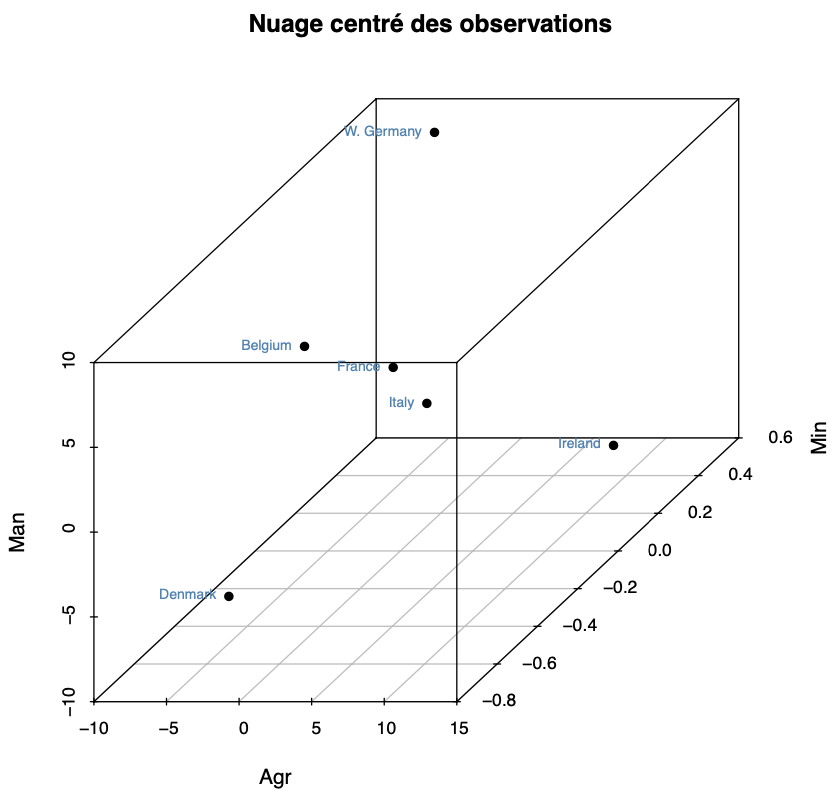
\includegraphics[scale = 0.52]{nuage_centre.png}
\end{figure}

\end{frame}

% ------------------------------------------------------------------------------------------------------------------------------

\begin{frame}{Importance de centrer les variables en ACP}
    
\begin{figure}
    \centering
    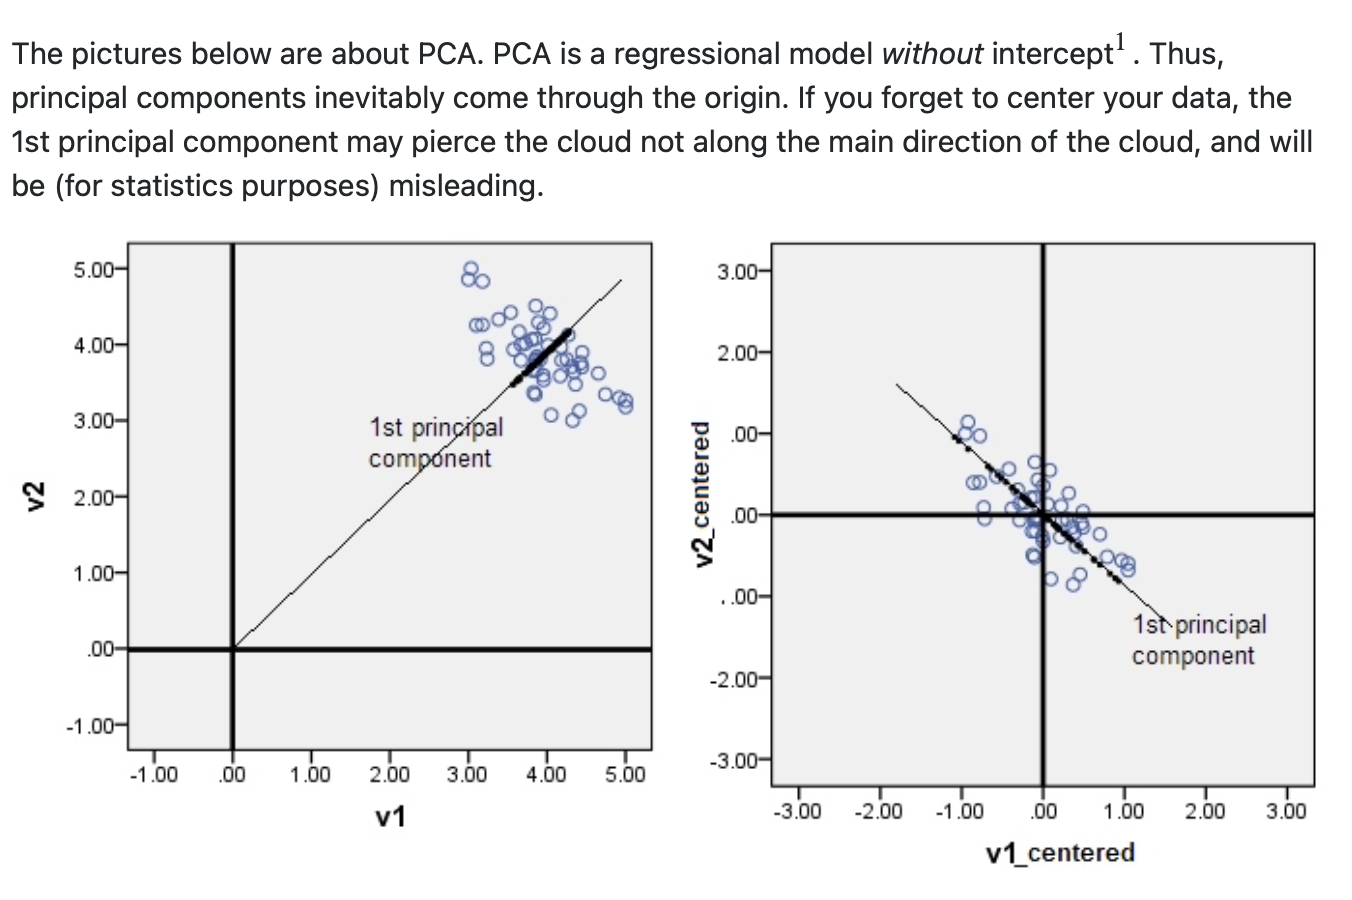
\includegraphics[scale = 0.45]{importance_centrer_nuage.png}
\end{figure}

\end{frame}

% ------------------------------------------------------------------------------------------------------------------------------

\begin{frame}{Nuage normalisé (centré-réduit) des observations}

\small
\begin{columns}[T]
    \begin{column}{0.48\textwidth}
        Matrice des données \motcle{originale} $\boldsymbol{X}$
        \begin{table}
            \centering
            \begin{tabular}{c|ccccc|}
                & 1 & \cdots & $j$ & \cdots & $p$\\
                \midrule
                1 &  &  &  &  & \\
                \vdots &  &  & \vdots &  & \\
                $i$ &  & \cdots & $x_{ij}$ & \cdots & \\
                \vdots &  &  & \vdots &  & \\
                $n$ &  &  &  &  & \\
                \midrule
                \midrule
                $\boldsymbol{\overline{x}}$ &  & \cdots & $\overline{x}^j$ & \cdots &\\
                $\boldsymbol{s}$ &  & \cdots & $s_j$ & \cdots &
            \end{tabular}
        \end{table}
    \end{column}
    \begin{column}{0.48\textwidth}
        Matrice des données \motcle{centrée-réduite} $\boldsymbol{Z}$
        \begin{table}
            \centering
            \begin{tabular}{c|ccccc|}
                & 1 & \cdots & $j$ & \cdots & $p$\\
                \midrule
                1 &  &  &  &  & \\
                \vdots &  &  & \vdots &  & \\
                $i$ &  & \cdots & $z_{ij}$ & \cdots & \\
                \vdots &  &  & \vdots &  & \\
                $n$ &  &  &  &  & \\
                \midrule
                \midrule
                $\boldsymbol{\overline{z}}$ &  & \cdots & $0$ & \cdots &\\
                $\boldsymbol{s}$ &  & \cdots & $1$ & \cdots &
            \end{tabular}
        \end{table}
    \end{column}
\end{columns}

Ici:
\begin{itemize}
    \fleche $s_j^2 = \frac{1}{n} \sum_{i = 1}^n (x_{ij} - \overline{x}^j)^2$ est la variance empirique de la $j^\text{e}$ variable,
    \fleche \motclef{$z_{ij} = \frac{x_{ij} - \overline{x}^j}{s_j}$} est le terme générique de la matrice centrée-réduite des données $\boldsymbol{Z}$.
    \fleche Les colonnes de la \motcle{matrice centrée-réduite $\boldsymbol{Z}$} ont une moyenne de 0 et une variance de 1:
    \begin{align*}
        \overline{z}^j = \frac{1}{n}\sum_{i = 1}^n z_{ij} = 0, \quad \text{Var}(\boldsymbol{z}^j) = \frac{1}{n}\sum_{i = 1}^n (z_{ij} - \overline{z}^j)^2 = \frac{1}{n} \sum_{i = 1}^n z_{ij}^2 = 1.
    \end{align*}
    \fleche Les distances entre les observations ne sont pas préservées, c'est-à-dire que
    \begin{align*}
        d_{\boldsymbol{M}}(\boldsymbol{x}_i, \boldsymbol{x}_j) \ne d_{\boldsymbol{M}}(\boldsymbol{z}_i, \boldsymbol{z}_j),
    \end{align*}
    où $d_{\boldsymbol{M}}(\cdot, \cdot)$ est une mesure de distance.
\end{itemize}

\end{frame}

% ------------------------------------------------------------------------------------------------------------------------------

\begin{frame}[fragile]{Nuage centré-réduit des observations}

\small
\textbf{Exemple:} jeu de données \texttt{eurojob}

\begin{code}
> # Centrer-réduire la matrice des données x
> ecart_type <- function(x) {sqrt(mean((x - mean(x))^2))}
> z <- x
> for(j in 1:ncol(x)) {
+     z[ , j] <- (x[ , j] - mean(x[ , j])) / ecart_type(x[ , j])
+ }
\end{code}

\begin{columns}[T]
    \begin{column}{0.45\textwidth}
        Matrice des données \motcle{originale} $\boldsymbol{X}$
        \begin{code}
> round(x, 4)
            Agr Min  Man
Belgium     3.3 0.9 27.6
Denmark     9.2 0.1 21.8
France     10.8 0.8 27.5
W. Germany  6.7 1.3 35.8
Ireland    23.2 1.0 20.7
Italy      15.9 0.6 27.6
        \end{code}
        Écart-type des colonnes de $\boldsymbol{X}$
        \begin{code}
> round(apply(x, 2, ecart_type), 4)
   Agr    Min    Man 
6.4847 0.3716 4.9155 
        \end{code}
    \end{column}
    \begin{column}{0.45\textwidth}
        Matrice des données \motcle{centrée-réduite} $\boldsymbol{Z}$
        \begin{code}
> round(z, 4)
               Agr     Min     Man
Belgium    -1.2671  0.3140  0.1560
Denmark    -0.3573 -1.8391 -1.0240
France     -0.1105  0.0449  0.1356
W. Germany -0.7428  1.3905  1.8242
Ireland     1.8017  0.5831 -1.2478
Italy       0.6759 -0.4934  0.1560
        \end{code}
        Écart-type des colonnes de $\boldsymbol{Z}$
        \begin{code}
> round(apply(z, 2, ecart_type), 4)
Agr Min Man 
  1   1   1
        \end{code}
    \end{column}
\end{columns}
    
\end{frame}

% ------------------------------------------------------------------------------------------------------------------------------

\begin{frame}{Nuage centré-réduit des observations}

Normaliser (centrer-réduire) les données s'interprète comme une translation suivie d'une normalisation du nuage des obseravtions dans $\mathbb{R}^p$.
    \begin{figure}
    \centering
    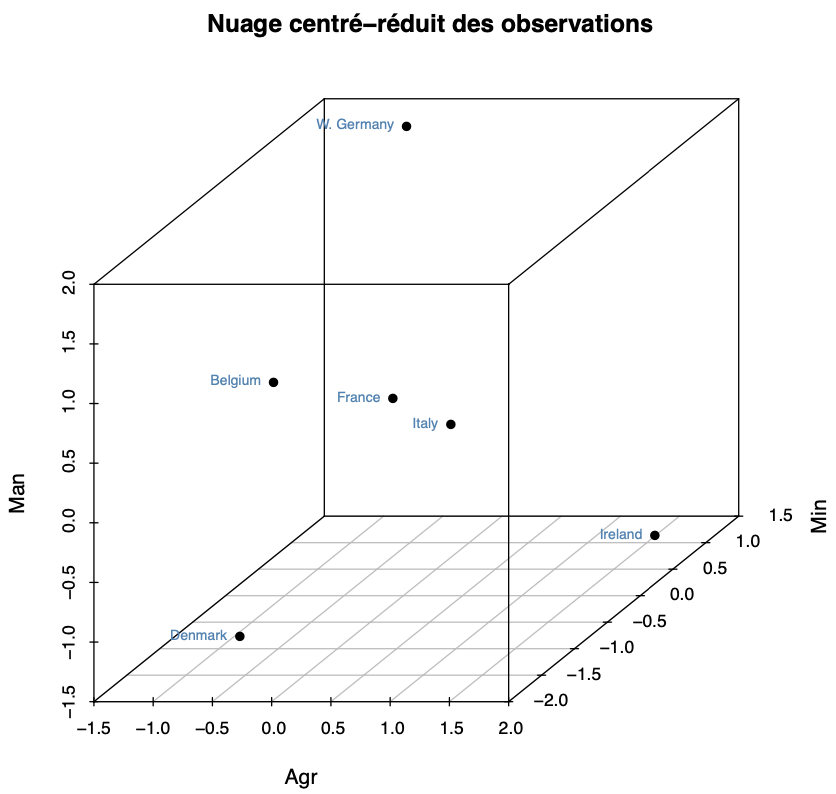
\includegraphics[scale = 0.52]{nuage_centre_reduit.png}
\end{figure}

\end{frame}

% ------------------------------------------------------------------------------------------------------------------------------

% ------------------------------------------------------------------------------------------------------------------------------

\begin{frame}{Distance entre 2 observations}
    
\begin{itemize}
    \fleche La proximité entre 2 observations peut être mesurée avec la \motcle{distance euclidienne}.
    \fleche La distance euclidienne entre 2 observations $i$ et $i'$ (2 lignes de $\boldsymbol{X}$) est
    \begin{align*}
        d_2(\boldsymbol{x}_i, \boldsymbol{x}_{i'}) = \sum_{i = 1}^p (x_{ij} - x_{i'j})^2.
    \end{align*}
    \fleche Quand les données sont \motcle{centrées-réduites}, la \motcle{distance euclidienne} entre 2 observations $\boldsymbol{z}_i$ et $\boldsymbol{z}_{i'}$ (2 lignes de $\boldsymbol{Z}$) est 
    \begin{align*}
        d_2(\boldsymbol{z}_i, \boldsymbol{z}_{i'}) = \sum_{i = 1}^p \frac{1}{s_j^2}(x_{ij} - x_{i'j})^2 = \sum_{i = 1}^p (z_{ij} - z_{i'j})^2.
    \end{align*}
\end{itemize}

\textbf{Cela signifie que:}

\begin{itemize}
    \fleche Si les variables (colonnes de $\boldsymbol{X}$) sont mesurées avec des \motcle{échelles différentes}, les variables avec des variances plus grandes seront plus importantes lors du calcul de la distance euclidienne.
    \fleche Normaliser les données permet de donner la \motcle{même importance} à toutes les variables lors du calcul de la distance.
    \fleche La plupart du temps, on utilise donc la \motcle{distance euclidienne} (métrique identité $\boldsymbol{M} = \boldsymbol{I}$) sur les \motcle{données centrées-réduites}.
\end{itemize}
    
\end{frame}

% ------------------------------------------------------------------------------------------------------------------------------

\begin{frame}{Inertie}

\small
\begin{itemize}
    \fleche L'\motcle{inertie} d'un nuage de points (ou d'observations) est une mesure de dispersion de ce même nuage. Elle est définie par 
    \begin{align*}
        \mathbb{I}(\boldsymbol{X}) = \sum_{i = 1}^n w_i d_{\boldsymbol{M}}^2(\boldsymbol{x}_i, \overline{\boldsymbol{x}}),
    \end{align*}
    où $\overline{\boldsymbol{x}} = (\overline{x}^1, \dots, \overline{x}^p)$ est le centre de gravité du nuage.
\end{itemize}

\begin{propo}
    \begin{itemize}
        \fleche Si on choisit une métrique diagonale $\boldsymbol{M} = \text{diag}(m_1, \dots, m_k)$ et $w_i = 1/n\quad \forall i$, on obtient 
        \begin{align*}
            \mathbb{I}(\boldsymbol{X}) = \sum_{j = 1}^p m_j \text{Var}(\boldsymbol{x}^j)
        \end{align*}
    \fleche En particulier, si on utilise $\boldsymbol{M} = \boldsymbol{I}$, alors 
    \begin{align*}
        \mathbb{I}(\boldsymbol{X}) = \sum_{j = 1}^p \text{Var}(\boldsymbol{x}^j) = \sum_{j = 1}^p s_j^2
    \end{align*}
    et
    \begin{align*}
         \mathbb{I}(\boldsymbol{Z}) = p.
    \end{align*}
    \end{itemize}
    *Faire la démonstration en exercice.
\end{propo}

\begin{itemize}
    \fleche On peut donc voir l'inertie comme une \motcle{variance généralisée} à plusieurs dimensions.
\end{itemize}

\end{frame}

% ------------------------------------------------------------------------------------------------------------------------------

\begin{frame}[fragile]{Inertie}

\small
\textbf{Exemple:} inertie du jeu de données \texttt{eurojob} (en supposant $w_i = 1/n \quad \forall i$ et $\boldsymbol{M} = \boldsymbol{I}$).
\vspace{0.3cm}
\begin{columns}
    \begin{column}{0.48\textwidth}
       Données \motcle{centrées} $\boldsymbol{Y}$
        \begin{code}
> round(y, 2)
             Agr   Min   Man
Belgium    -8.22  0.12  0.77
Denmark    -2.32 -0.68 -5.03
France     -0.72  0.02  0.67
W. Germany -4.82  0.52  8.97
Ireland    11.68  0.22 -6.13
Italy       4.38 -0.18  0.77
        \end{code}
        Variances des colonnes
        \begin{code}
> round(apply(x, 2, ecart_type) ^ 2, 4)
    Agr     Min     Man 
42.0514  0.1381 24.1622 
        \end{code}
    \end{column}
    \begin{column}{0.48\textwidth}
        Données \motcle{centrées-réduites} $\boldsymbol{Z}$
        \begin{code}
> round(z, 2)
             Agr   Min   Man
Belgium    -1.27  0.31  0.16
Denmark    -0.36 -1.84 -1.02
France     -0.11  0.04  0.14
W. Germany -0.74  1.39  1.82
Ireland     1.80  0.58 -1.25
Italy       0.68 -0.49  0.16
        \end{code}
        Variance des colonnes
        \begin{code}
> round(apply(z, 2, ecart_type) ^ 2, 4)
Agr Min Man 
  1   1   1 
        \end{code}
    \end{column}
\end{columns}

\begin{itemize}
    \fleche Inertie du jeu de données \motcle{centré}:
    \begin{align*}
        I(\boldsymbol{Y}) = 42.0514 + 0.1381 + 24.1622 = 70.3517.
    \end{align*}
    \fleche Inertie du jeu de données \motcle{centré-réduit}:
    \begin{align*}
        I(\boldsymbol{Z}) = 1 + 1 + 1 = 3.
    \end{align*}
\end{itemize}

\end{frame}

% ------------------------------------------------------------------------------------------------------------------------------

\subsection{Nuage des variables}

% ------------------------------------------------------------------------------------------------------------------------------

\begin{frame}[fragile]{Nuage des variables}

\textbf{Exemple:} les 3 industries d'\texttt{eurojob} (Agr, Min et Man) définissent un nuage de $p = 3$ points dans $\mathbb{R}^6$. On ne peut pas visualiser ce nuage de points, car il est en 6 dimensions.
\small
\begin{code}
> t(x)
    Belgium Denmark France W. Germany Ireland Italy
Agr     3.3     9.2   10.8        6.7    23.2  15.9
Min     0.9     0.1    0.8        1.3     1.0   0.6
Man    27.6    21.8   27.5       35.8    20.7  27.6
\end{code}
\normalsize
\begin{itemize}
    \fleche Chaque variable $j$ est un point $\boldsymbol{x}^j$ dans $\mathbb{R}^n$ (une colonne de $\boldsymbol{X}$).
    \fleche Un poids $m_j$ est associé à chaque variable $j$.
    \begin{itemize}
        \item[-] $m_j = 1$ en ACP.
        \item[-] $m_j \ne 1$ en analyse des correspondances multiples.
    \end{itemize}
\end{itemize}


\begin{itemize}
    \fleche Quand les données sont centrées:
    \begin{itemize}
        \item[-] chaque variable $j$ est un point noté $\boldsymbol{y}^j$ dans $\mathbb{R}^n$,
        \item[-] on parle des variables centrées.
    \end{itemize}
    \fleche Quand les données sont centrées-réduites:
    \begin{itemize}
        \item[-] chaque variable $j$ est un point noté $\boldsymbol{z}^j$ dans $\mathbb{R}^n$,
        \item[-] on parle des variables normalisées.
    \end{itemize}
\end{itemize}
    
\end{frame}

% ------------------------------------------------------------------------------------------------------------------------------

\begin{frame}{Lien entre 2 variables}

Il n'est pas naturel de parler de distance entre 2 variables. On mesure plutôt le lien entre 2 variables en utilisant la \motcle{covariance} ou la \motcle{corrélation} empiriques.

\begin{itemize}
    \fleche Pour définir la covariance et la corrélation, un métrique $\boldsymbol{N}$ est introduite dans l'espace $\mathbb{R}^n$:
    \begin{align*}
        \boldsymbol{N} = \text{diag}(1/n, \dots, 1/n).
    \end{align*}
    \begin{itemize}
        \item[-] Cette métrique est la plus naturelle à utiliser pour cet espace puisqu'elle nous permet d'exprimer certaines quantités (écart-type, variance, covariance, corrélation, etc.) en termes de produits scalaires.
    \end{itemize}
    \fleche Le produit scalaire entre $\boldsymbol{x}$ et $\boldsymbol{y}$ dans $\mathbb{R}^n$ est défini par 
    \begin{align*}
        \langle \boldsymbol{x}, \boldsymbol{y} \rangle_{\boldsymbol{N}} = \boldsymbol{x}^\top \boldsymbol{N} \boldsymbol{y} = \frac{1}{n} \boldsymbol{x}^\top \boldsymbol{y} = \frac{1}{n}\sum_{i = 1}^n x_i y_i.
    \end{align*}
    \fleche La norme de $\boldsymbol{x}$ dans $\mathbb{R}^n$ est alors
    \begin{align*}
        ||\boldsymbol{x}||_{\boldsymbol{N}} = \sqrt{\langle \boldsymbol{x}, \boldsymbol{x} \rangle_{\boldsymbol{N}}} = \sqrt{\frac{1}{n} \sum_{i = 1}^n x_i^2}.
    \end{align*}
\end{itemize}

\end{frame}

% ------------------------------------------------------------------------------------------------------------------------------

\begin{frame}{Variance, covariance et corrélation}

\begin{itemize}
    \fleche Avec cette métrique, la \motcle{variance} peut s'écrire comme une \motcle{norme au carré}:
    \begin{itemize}
        \blt $\text{Var}(\boldsymbol{x}^j) = \frac{1}{n}\sum_{i = 1}^n (x_{ij} - \overline{x}^j)^2 = ||\boldsymbol{y}^j||_{\boldsymbol{N}}^2$,
        \blt $\text{Var}(\boldsymbol{z}^j) = \frac{1}{n}\sum_{i = 1}^n (z_{ij} - \overline{z}^j)^2 = ||\boldsymbol{z}^j||_{\boldsymbol{N}}^2$ = 1.
    \end{itemize}
    \fleche Les $p$ variables sont donc situées sur la sphère unitaire de $\mathbb{R}^n$ (puisque $||\boldsymbol{z}^j||_{\boldsymbol{N}} = 1$).
    \fleche De plus, la \motcle{covariance} et la \motcle{corrélation} s'expriment comme un produit scalaire:
    \begin{itemize}
        \blt $c_{j, j'} = \frac{1}{n} \sum_{i = 1}^n(x_{ij} - \overline{x}^j)(x_{ij'} - \overline{x}^{j'}) = \langle \boldsymbol{y}^j, \boldsymbol{y}^{j'}\rangle_{\boldsymbol{N}}$,
        \blt $r_{j, j'} = \frac{1}{n} \sum_{i = 1}^n\left(\frac{x_{ij} - \overline{x}^j}{s_j}\right)\left(\frac{x_{ij'} - \overline{x}^{j'}}{s_{j'}}\right) = \langle \boldsymbol{z}^j, \boldsymbol{z}^{j'}\rangle_{\boldsymbol{N}}$.
    \end{itemize}
    \fleche Ceci conduit à une expression simple de la matrice de covariance notée $\boldsymbol{C}$ et de la matrice de corrélation notée $\boldsymbol{R}$:
    \begin{itemize}
        \blt $\boldsymbol{C} = \boldsymbol{Y}^\top \boldsymbol{N}\boldsymbol{Y}$,
        \blt $\boldsymbol{R} = \boldsymbol{Z}^\top \boldsymbol{N}\boldsymbol{Z}$.
    \end{itemize}
\end{itemize}

\end{frame}

% ------------------------------------------------------------------------------------------------------------------------------

\begin{frame}{Interprétation géométrique de la corrélation entre 2 variables}

\begin{itemize}
    \fleche Avec la métrique $\boldsymbol{N}$, la \motcle{corrélation} entre 2 variables s'écrit comme le \motcle{cosinus de l'angle} entre celles-ci:
    \begin{itemize}
        \blt $r_{jj'} = \frac{\langle \boldsymbol{y}^j, \boldsymbol{y}^{j'}\rangle_{\boldsymbol{N}}}{||\boldsymbol{y}^j||_{\boldsymbol{N}} ||\boldsymbol{y}^{j'}||_{\boldsymbol{N}}} = \cos[\theta(\boldsymbol{y}^j, \boldsymbol{y}^{j'})]$,
        \blt $r_{jj'} = \langle \boldsymbol{z}^j, \boldsymbol{z}^{j'}\rangle_{\boldsymbol{N}} = \cos[\theta(\boldsymbol{z}^j, \boldsymbol{z}^{j'})]$.
    \end{itemize}
    \fleche Ceci nous permet d'avoir une \motcle{interprétation géométrique de la corrélation} entre 2 variables:
     \begin{itemize}
        \item[-] un angle droit (90 degrés ou $\pi/2$ radians) correspond à une corrélation nulle;
        \item[-] un angle nul correspond à une corrélation de 1; et
        \item[-] un angle plat (180 degrés ou $\pi$ radians) correspond à une corrélation de -1.
    \end{itemize}
\end{itemize}

\end{frame}

% ------------------------------------------------------------------------------------------------------------------------------

\begin{frame}{En bref}
    
\begin{itemize}
    \fleche Une ACP peut se faire à partir
    \begin{itemize}
        \item[-] des données centrées $\boldsymbol{Y}$; ou 
        \item[-] des données centrées-réduites $\boldsymbol{Z}$.
    \end{itemize}
    \fleche Ceci conduit à 2 types d'ACP:
    \begin{itemize}
        \item[-] l'ACP non standardisée (ou ACP sur la matrice de covariance), qui analyse $\boldsymbol{Y}$,
        \item[-] l'ACP standardisée (ou ACP sur la matrice de corrélation), qui analyse $\boldsymbol{Z}$.
    \end{itemize}
    \fleche Une ACP se fait en étudiant 2 nuages: le nuage des $n$ \motcle{observations} dans $\mathbb{R}^p$ avec la métrique $\boldsymbol{M}$ (en pratique, on prend $\boldsymbol{M} = \boldsymbol{I}_p$) et le nuage des $p$ \motcle{variables} dans $\mathbb{R}^n$ avec la métrique $\boldsymbol{N} = (1/n)\boldsymbol{I}_n$.
\end{itemize}

\textbf{À partir de maintenant, nous ne considérerons que l'ACP standardisée en utilisant la métrique $\boldsymbol{I}_p$ pour le nuage des observations et la métrique $\boldsymbol{N} = (1/n)\boldsymbol{I}_n$ pour le nuage des variables.}
    
\end{frame}

% ------------------------------------------------------------------------------------------------------------------------------

\section{Analyse du nuage des observations}

% ------------------------------------------------------------------------------------------------------------------------------

\begin{frame}{Analyse du nuage des observations}
    
\begin{exampleblock}{Objectif}
    \begin{itemize}
        \fleche Trouver un espace (ici un plan) tel que les distances entre les observations soient les mieux préservées.
    \end{itemize}
\end{exampleblock}

\begin{figure}
    \centering
    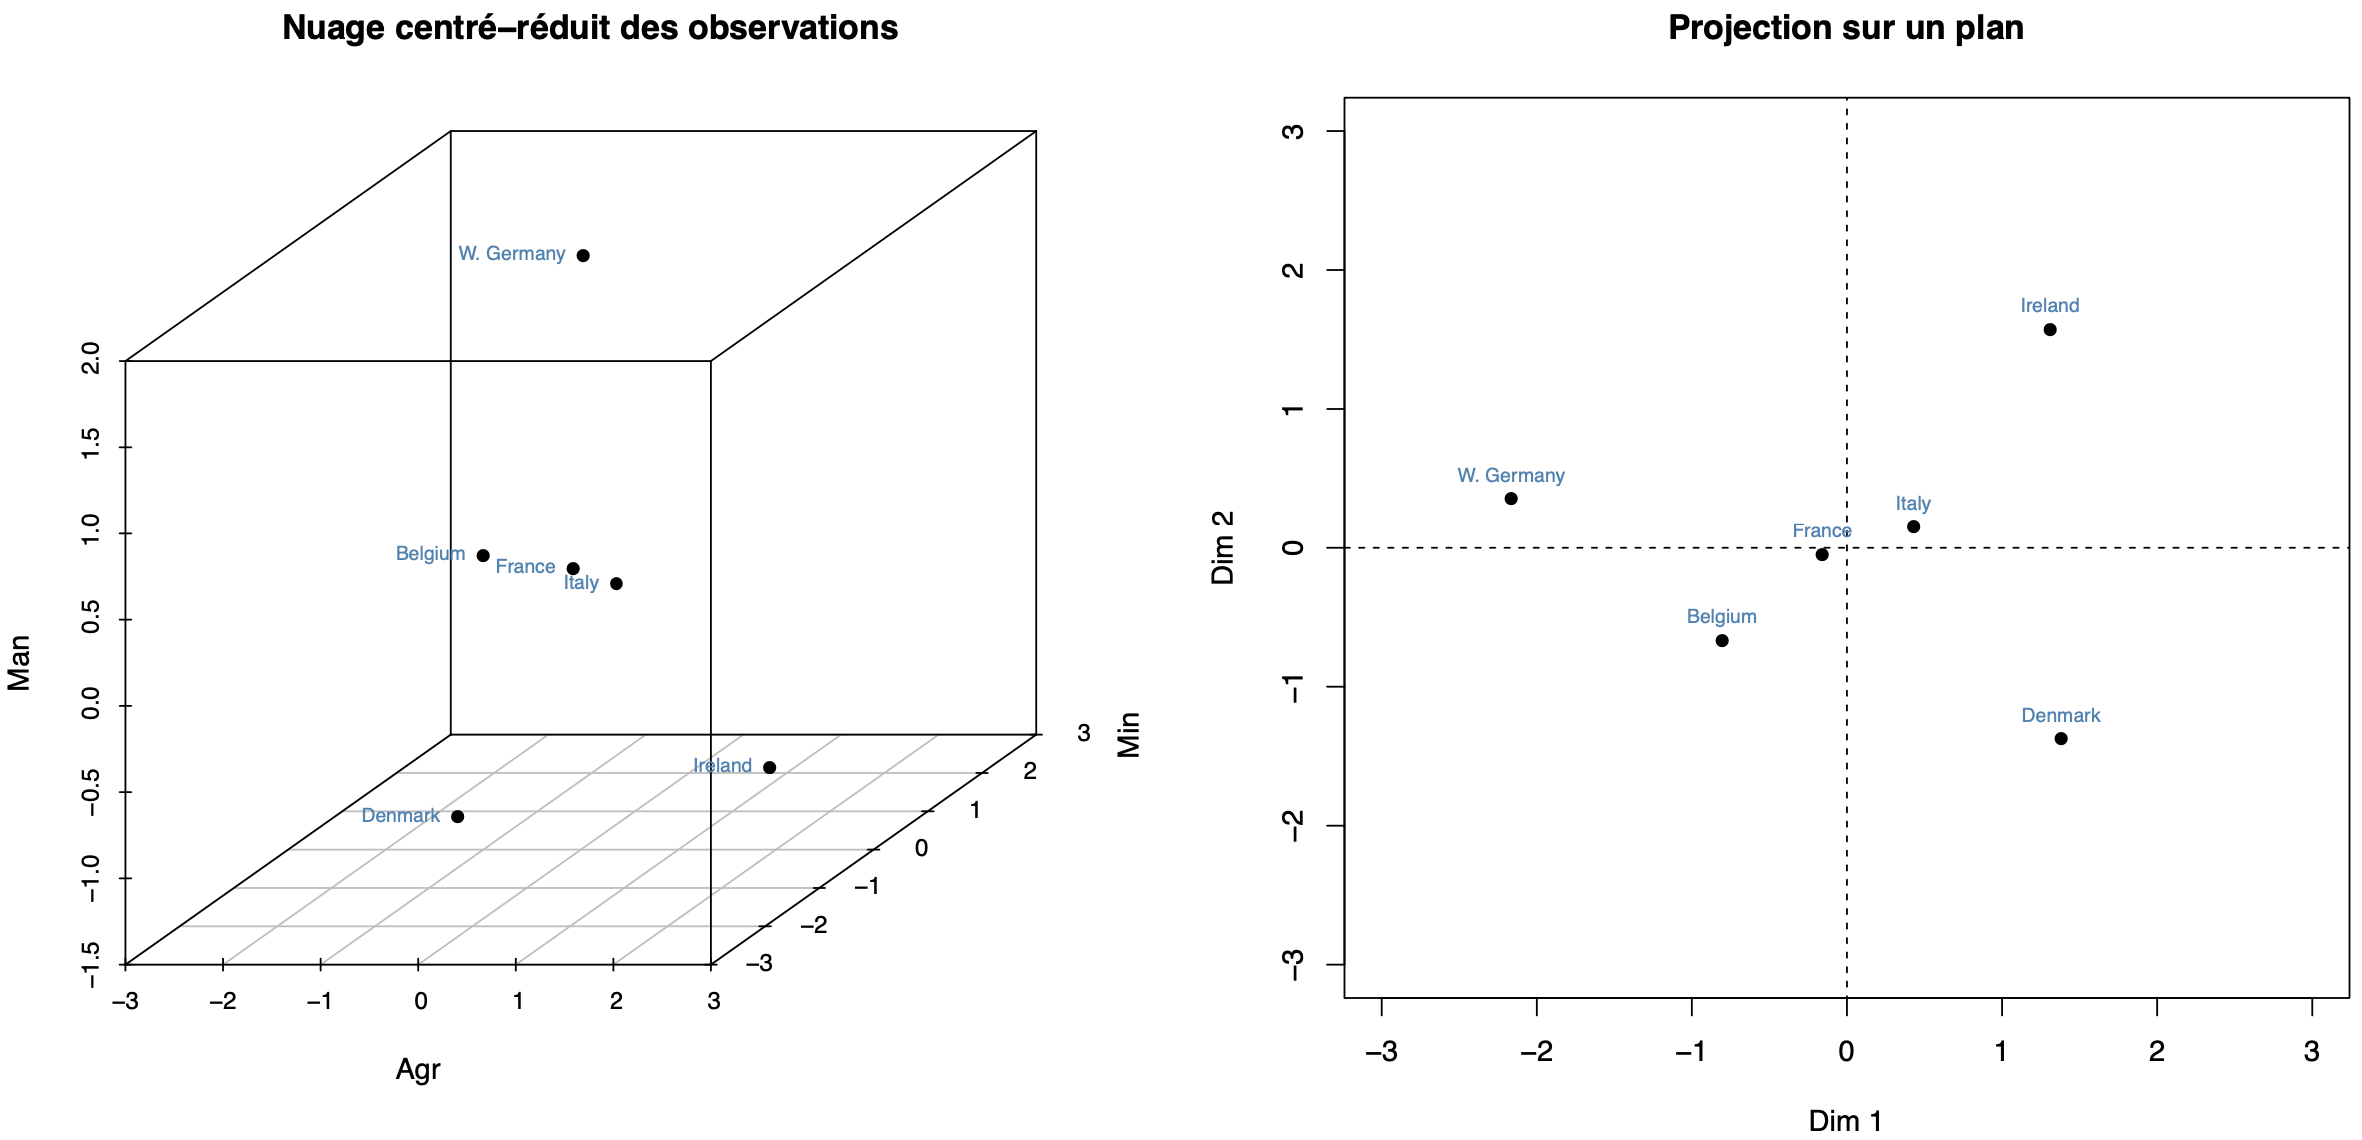
\includegraphics[scale = 0.25]{nuage_projection.png}
\end{figure}

\end{frame}

% ------------------------------------------------------------------------------------------------------------------------------

\begin{frame}{Projection d'une observation sur un axe}


\begin{itemize}
    \fleche La \motcle{coordonée de la projection} orthogonale d'un point $\boldsymbol{z}_i \in \mathbb{R}^p$ sur un axe $\boldsymbol{\Delta}_\alpha$ défini par le vecteur unitaire $\boldsymbol{v}_\alpha$ ($\boldsymbol{v}_\alpha^\top \boldsymbol{v}_\alpha = 1$) est:
    \begin{align*}
        f_{i\alpha} = \langle \boldsymbol{z}_i, \boldsymbol{v}_\alpha \rangle = \boldsymbol{z}_i^\top \boldsymbol{v}_\alpha.
    \end{align*}
     \fleche Pour s'en convaincre, se souvenir que $\langle \boldsymbol{x}, \boldsymbol{y} \rangle$ est la \motcle{norme} du \motcle{vecteur $\boldsymbol{x}$ projeté orthogonalement sur le vecteur $\boldsymbol{y}$} multipliée par la \motcle{norme de $\boldsymbol{x}$}.
    \fleche Le \motcle{vecteur des coordonées} sur l'axe $\boldsymbol{\Delta}_\alpha$ pour les $n$ observations est:
    \begin{align*}
        \boldsymbol{f}^\alpha = \begin{pmatrix} f_{1\alpha} \\ \vdots \\ f_{n\alpha} \end{pmatrix} = \boldsymbol{Z}\boldsymbol{v}_\alpha = \sum_{i = 1}^p v_{j\alpha} \boldsymbol{z}^j.
    \end{align*}
    \begin{itemize}
        \blt $\boldsymbol{f}^\alpha$ est une \motcle{combinaison linéaire} des colonnes de $\boldsymbol{Z}$.
        \blt $\boldsymbol{f}^\alpha$ est \motcle{centré} (en supposant que les colonnes de $\boldsymbol{Z}$ soient centrées).
    \end{itemize}
\end{itemize}

En ACP, les vecteurs $\boldsymbol{v}_1, \boldsymbol{v}_2, \dots$ sont choisis de manière à \motcle{maximiser l'inertie des projections} des observations.

\end{frame}

% ------------------------------------------------------------------------------------------------------------------------------

\begin{frame}{Projection d'une observation sur un axe -- Exemple}

\small 
\begin{exemple}
    \begin{itemize}
        \fleche On considère la matrice \texttt{eurojob} centrée-réduite
        \begin{align*}
            \boldsymbol{Z} = 
            \begin{bmatrix}
                -1.2671 & 0.3140 & 0.1560 \\ 
                -0.3573 & -1.8391 & -1.0240 \\ 
                -0.1105 & 0.0449 & 0.1356 \\ 
                -0.7428 & 1.3905 & 1.8242 \\ 
                1.8017 & 0.5831 & -1.2478 \\ 
                0.6759 & -0.4934 & 0.1560 \\ 
            \end{bmatrix}
        \end{align*}
        \fleche On veut projeter les 6 observations sur les axes orthogonaux $\boldsymbol{\Delta}_1$ et $\boldsymbol{\Delta}_2$ définis respectivement par les vecteurs unitaires
        \begin{align*}
            \boldsymbol{v}_1 = \begin{bmatrix} -0.4783158 \\ 0.5237373 \\ 0.7049207 \end{bmatrix}\quad \text{et}\quad
            \boldsymbol{v}_2 = \begin{bmatrix} 0.739170360 \\ 0.673517525 \\ 0.00114991 \end{bmatrix}.
        \end{align*}
        \fleche Calculer $\boldsymbol{f}^1$ et $\boldsymbol{f}^2$.
    \end{itemize}
\end{exemple}

\textbf{Réponse:}

$\boldsymbol{f}^1 = \boldsymbol{Z}\boldsymbol{v}_1$ et $\boldsymbol{f}^2 = \boldsymbol{Z}\boldsymbol{v}_2$.
\begin{itemize}
    \fleche $\boldsymbol{f}^1$ nous donne les coordonnées des 6 observations projetées sur l'axe définit par $\boldsymbol{v}_1$.
    \fleche $\boldsymbol{f}^2$ nous donne les coordonnées des 6 observations projetées sur l'axe définit par $\boldsymbol{v}_2$.
\end{itemize}

\end{frame}

% ------------------------------------------------------------------------------------------------------------------------------

\begin{frame}{Sélection des vecteurs $\boldsymbol{v}$}

\begin{itemize}
    \fleche Dans un \motcle{premier temps}, on cherche un axe $\boldsymbol{\Delta}_1$ défini par un vecteur unitaire $\boldsymbol{v}_1\in\mathbb{R}^p$ tel que
    \begin{align*}
        \boldsymbol{v}_1 &= \argmax{||\boldsymbol{v}|| = 1} \text{Var}(\boldsymbol{Z}\boldsymbol{v}) \\
        &= \argmax{||\boldsymbol{v}|| = 1} \boldsymbol{v}^\top \boldsymbol{R} \boldsymbol{v},
    \end{align*}
    où \begin{align*}
        \boldsymbol{R} = \frac{1}{n}\boldsymbol{Z}^\top \boldsymbol{Z} \in \mathbb{R}^{p\times p}
    \end{align*}
     est la matrice de corrélation.
    \fleche On cherche donc l'axe $\boldsymbol{\Delta}_1$ qui \motcle{maximize la variance des observations projetées} sur ce même axe.
\end{itemize}

\begin{itemize}
    \fleche On peut montrer que:
    \begin{itemize}
        \blt $\boldsymbol{v}_1$ est le \motcle{vecteur propre} associé à la \motcle{plus grande} valeur propre $\lambda_1$ de $\boldsymbol{R}$,
        \blt La \motcle{première composante principale} (PC1) $\boldsymbol{f}^1 = \boldsymbol{Z}\boldsymbol{v}_1$ est centrée:
        \begin{align*}
            \overline{\boldsymbol{f}^1} = 0,
        \end{align*}
        \blt $\lambda_1$ est la \motcle{variance} de la PC1:
        \begin{align*}
            \text{Var}(\boldsymbol{f}^1) = \lambda_1.
        \end{align*}
    \end{itemize}
\end{itemize}

\end{frame}

% ------------------------------------------------------------------------------------------------------------------------------

\begin{frame}{Sélection des vecteurs $\boldsymbol{v}$}

\begin{itemize}
    \fleche Dans un \motcle{second temps}, on cherche un axe $\boldsymbol{\Delta}_2$ défini par un vecteur $\boldsymbol{v}_2\in\mathbb{R}^p$ tel que
     \begin{align*}
        \boldsymbol{v}_2 &= \argmax{||\boldsymbol{v}|| = 1; \boldsymbol{v} \perp \boldsymbol{v}_1} \text{Var}(\boldsymbol{Z}\boldsymbol{v})\\
        &= \argmax{||\boldsymbol{v}|| = 1; \boldsymbol{v} \perp \boldsymbol{v}_1} \boldsymbol{v}^\top \boldsymbol{R}\boldsymbol{v}.
    \end{align*}
    \fleche On cherche donc l'axe $\boldsymbol{\Delta}_2$ \motcle{orthogonal} au premier axe principal ($\boldsymbol{\Delta}_1$) qui \motcle{maximise la variance des observations projetées} sur ce même axe.
    \fleche On peut montrer que:
        \begin{itemize}
        \blt $\boldsymbol{v}_2$ est le \motcle{vecteur propre} associé à la \motcle{deuxième plus grande} valeur propre $\lambda_2$ de $\boldsymbol{R}$,
        \blt La \motcle{deuxième composante principale} (PC2) $\boldsymbol{f}^2 = \boldsymbol{Z}\boldsymbol{v}_2$ est centrée:
        \begin{align*}
            \overline{\boldsymbol{f}^2} = 0,
        \end{align*}
        \blt $\lambda_2$ est la \motcle{variance} de la PC2:
        \begin{align*}
            \text{Var}(\boldsymbol{f}^2) = \lambda_2.
        \end{align*}
        \fleche Les composantes principales $\boldsymbol{f}^1$ et $\boldsymbol{f}^2$ ne sont pas corrélées.
    \end{itemize}
\end{itemize}

En continuant, on peut obtenir $q \le r$ (r est le rang de $\boldsymbol{Z}$) axes orthogonaux $\boldsymbol{\Delta}_1, \dots, \boldsymbol{\Delta}_q$ sur lesquels les observations sont projetées orthogonalement.
    
\end{frame}

% ------------------------------------------------------------------------------------------------------------------------------

\begin{frame}{En résumé}

\begin{itemize}
    \item[1.] La \motcle{décomposition spectrale} de la matrice $\boldsymbol{R}$ est effectuée et $q \le r$ est choisi.
    \item[2.] La matrice $\boldsymbol{F} = \boldsymbol{Z}\boldsymbol{V}\in \mathbb{R}^{n \times q}$ des \motclef{$q$ composantes principales} est obtenue, où $\boldsymbol{V}$ est la matrice des $q$ premiers vecteurs propres de $\boldsymbol{R}.$
    \begin{itemize}
        \item[-] Les composantes principales $\boldsymbol{f}^\alpha = \boldsymbol{Z}\boldsymbol{v}_\alpha, \alpha = 1, \dots, q$ (colonnes de $\boldsymbol{F}$) sont centrées et de variance $\lambda_\alpha$.
        \item[-] Les éléments $f_{i\alpha}$ sont appelés les \og{}factor coordinates\fg{} ou les \og{}scores\fg{} des observations sur les composantes principales.
    \end{itemize}
\end{itemize}


\begin{table}
    \centering
    $\boldsymbol{F} = $
    \begin{tabular}{c|ccccc|}
        & 1 & \cdots & $\alpha$ & \cdots & $q$\\
        \midrule
        1 &  &  &  &  & \\
        \vdots &  &  & \vdots &  & \\
        $i$ &  & \cdots & $f_{i\alpha}$ & \cdots & \\
        \vdots &  &  & \vdots &  & \\
        $n$ &  &  &  &  & \\
        \midrule
        \midrule
        moyenne &  & \cdots & $0$ & \cdots &\\
        variance &  & \cdots & $\lambda_\alpha$ & \cdots &
    \end{tabular}
\end{table}
    
\end{frame}

% ------------------------------------------------------------------------------------------------------------------------------

\begin{frame}[fragile]{Exemple}

\small
\textbf{Exemple:} matrice $\boldsymbol{F}$ des $q = 2$ premières composantes de l'extrait du jeu de données \texttt{eurojob}.

\begin{code}
> acp$ind$coord[ , 1:2]
                Dim.1       Dim.2
Belgium     0.8804620 -0.72493205
Denmark    -1.5141449 -1.50391377
France      0.1719596 -0.05132316
W. Germany  2.3694452  0.38961453
Ireland    -1.4359290  1.72305846
Italy      -0.4717928  0.16749598
\end{code}

\begin{figure}
    \centering
    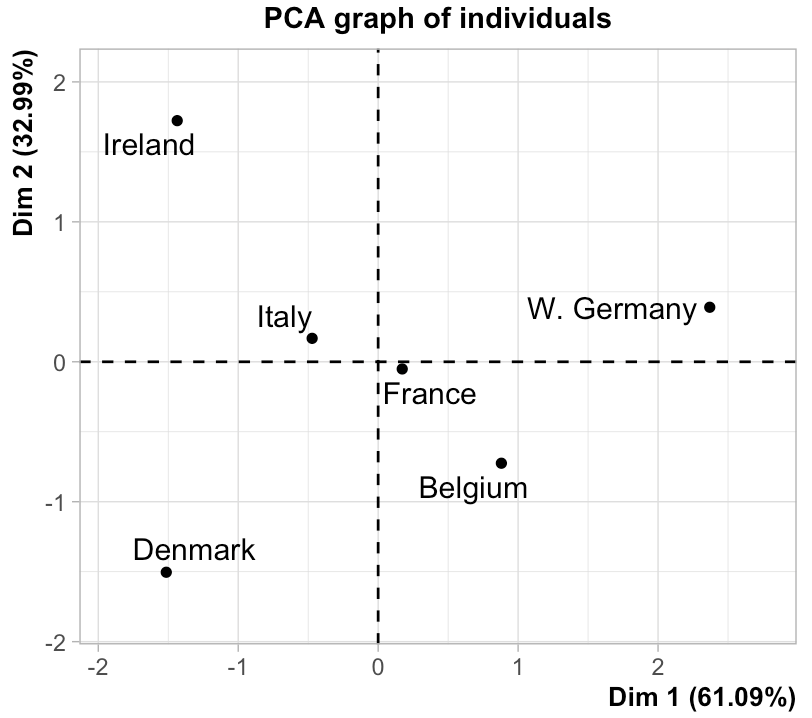
\includegraphics[scale = 0.37]{projection_plan.png}
\end{figure}
    
\end{frame}

% ------------------------------------------------------------------------------------------------------------------------------

\section{Analyse du nuage des variables}

% ------------------------------------------------------------------------------------------------------------------------------

\begin{frame}[fragile]{Analyse du nuage des variables}

\small
\begin{itemize}
    \fleche Les 3 variables centrées-réduites forment un nuage dans $\mathbb{R}^6$, et plus spécifiquement, dans l'\motcle{hypersphère de rayon 1}.
\end{itemize}

\begin{code}
> round(t(z), 4)
    Belgium Denmark  France W. Germany Ireland   Italy
Agr -1.2671 -0.3573 -0.1105    -0.7428  1.8017  0.6759
Min  0.3140 -1.8391  0.0449     1.3905  0.5831 -0.4934
Man  0.1560 -1.0240  0.1356     1.8242 -1.2478  0.1560
\end{code}

    
\begin{exampleblock}{Objectif}
    \begin{itemize}
        \fleche Trouver un espace (souvent un plan) tel que les angles entre les variables (c'est-à-dire les corrélations) soient les mieux préservées.
    \end{itemize}
\end{exampleblock}


\begin{columns}[T]
    \begin{column}{0.48\textwidth}
        \begin{figure}
            \centering
            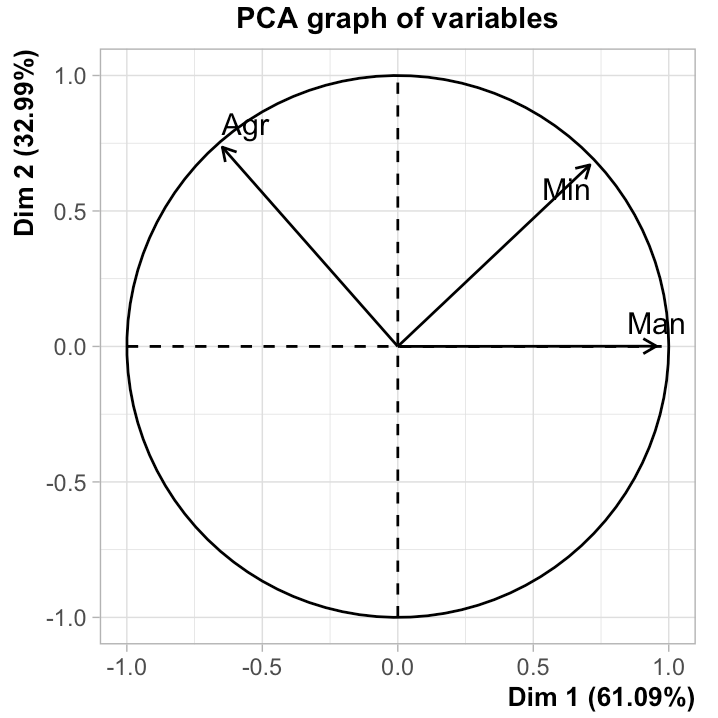
\includegraphics[scale = 0.3]{projection_variables_plan.png}
        \end{figure}
    \end{column}
    \begin{column}{0.48\textwidth}
        \begin{figure}
            \centering
            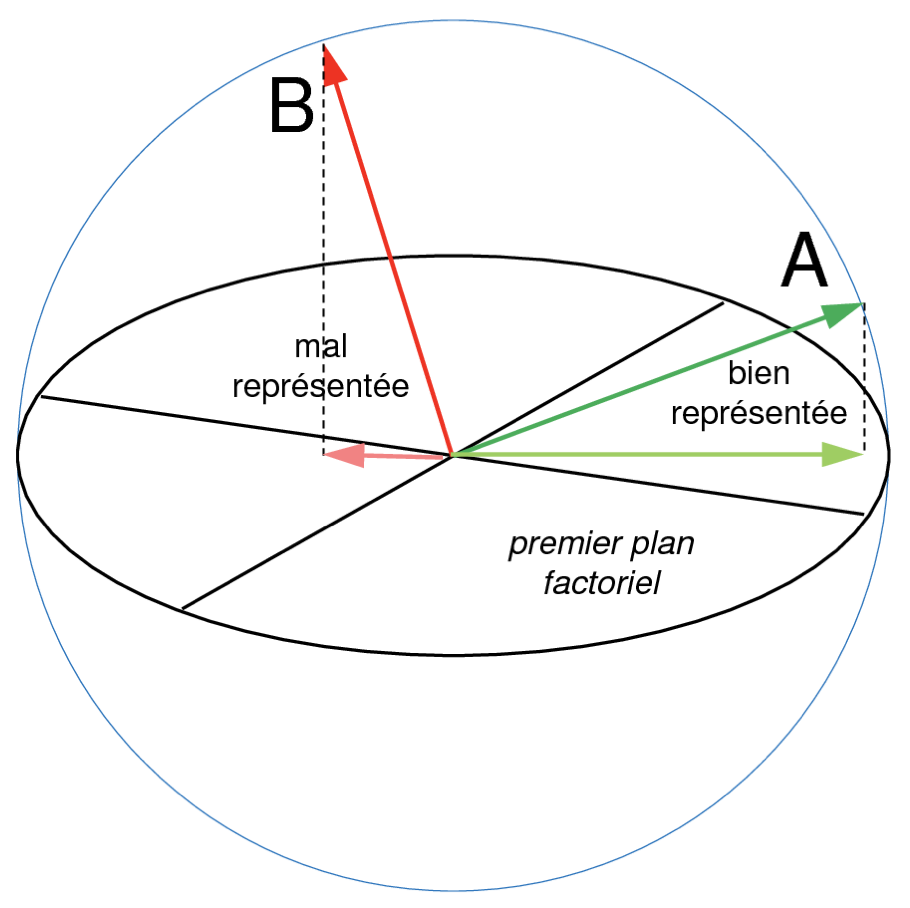
\includegraphics[scale = 0.22]{sphere_unite.png}
        \end{figure}
    \end{column}
\end{columns}

\end{frame}

% ------------------------------------------------------------------------------------------------------------------------------

\begin{frame}[fragile]{Projection d'une variable sur un axe}

\begin{itemize}
    \fleche La \motcle{coordonnée de la projection} $\boldsymbol{N}$-orthogonale d'un point $\boldsymbol{z}^j\in\mathbb{R}^n$ sur un axe $G_\alpha$ défini par le vecteur unitaire $\boldsymbol{u}_\alpha$ ($\boldsymbol{u}_\alpha^\top \boldsymbol{N} \boldsymbol{u}_\alpha = 1$) est:
    \begin{align*}
        a_{j\alpha} = \langle \boldsymbol{z}^j, \boldsymbol{u}_\alpha \rangle_{\boldsymbol{N}} = (\boldsymbol{z}^j)^\top \boldsymbol{N}\boldsymbol{u}_\alpha,
    \end{align*}
    \fleche Le \motcle{vecteur des coordonnées} sur l'axe $G_\alpha$ pour les $p$ variables est:
    \begin{align*}
        \boldsymbol{a}^\alpha = \begin{pmatrix} a_{1\alpha} \\ \vdots \\ a_{p\alpha} \end{pmatrix} = \boldsymbol{Z}^\top \boldsymbol{N}\boldsymbol{u}_\alpha.
    \end{align*}
\end{itemize}

En ACP, les vecteurs $\boldsymbol{u}_1, \boldsymbol{u}_2, \dots$ sont choisis de manière à \motcle{maximiser la somme des cosinus carrés des angles} entre les variables et l'axe de projection.

\begin{alertblock}{Attention: une métrique $\boldsymbol{N}$ dans $\mathbb{R}^n$ est utilisée}
\begin{itemize}
    \fleche Une métrique dans $\mathbb{R}^n$ est une matrice $n \times n$ semi-définie positive.
    \fleche Ici en ACP, $\boldsymbol{N}$ est la matrice diagonale des poids des observations:
    \begin{align*}
        \boldsymbol{N} = \text{diag}(w_1, \dots, w_n).
    \end{align*}
    \fleche Dans le cadre du cours, on ne considère que le cas où les observations ont le même poids $1/n$. On utilise donc la métrique $\boldsymbol{N} = \frac{1}{n}\boldsymbol{I}_n$.
\end{itemize}
\end{alertblock}

\end{frame}

% ------------------------------------------------------------------------------------------------------------------------------

\begin{frame}[fragile]{Projection d'une variable sur un axe -- Exemple}

\small 
\begin{exemple}
    \begin{itemize}
        \fleche On considère la matrice \texttt{eurojob} centrée-réduite
        \begin{align*}
            \boldsymbol{Z} = 
            \begin{bmatrix}
                -1.2671 & 0.3140 & 0.1560 \\ 
                -0.3573 & -1.8391 & -1.0240 \\ 
                -0.1105 & 0.0449 & 0.1356 \\ 
                -0.7428 & 1.3905 & 1.8242 \\ 
                1.8017 & 0.5831 & -1.2478 \\ 
                0.6759 & -0.4934 & 0.1560 \\ 
            \end{bmatrix}
        \end{align*}
        \fleche On veut projeter les 3 variables (en utilisant la métrique $\boldsymbol{N} = (1/6)\boldsymbol{I}_6$) sur les axes orthogonaux $G_1$ et $G_2$ définis respectivement par les vecteurs unitaires
         \begin{align*}
            \boldsymbol{u}_1 = 
            \begin{bmatrix}
                0.2655155 \\ 
                -0.4566114 \\ 
                0.0518568 \\ 
                0.7145390 \\ 
                -0.4330243 \\ 
                -0.1422757 \\ 
            \end{bmatrix}
            \quad \text{et}\quad
            \boldsymbol{u}_2 = 
            \begin{bmatrix}
                -0.2974757 \\ 
                -0.6171307 \\ 
                -0.0210604 \\ 
                0.1598782 \\ 
                0.7070567 \\ 
                0.0687319 \\ 
            \end{bmatrix}
        \end{align*}
        \fleche Calculer $\boldsymbol{a}^1$ et $\boldsymbol{a}^2$.
    \end{itemize}
\end{exemple}

\textbf{Réponse:}

\begin{itemize}
    \fleche $\boldsymbol{a}^1 = \boldsymbol{Z}^\top\boldsymbol{N}\boldsymbol{u}_1$ nous donne les coordonnées des 3 variables projetées sur l'axe définit par $\boldsymbol{u}_1$.
    \fleche $\boldsymbol{a}^2 = \boldsymbol{Z}^\top\boldsymbol{N}\boldsymbol{u}_2$ nous donne les coordonnées des 3 variables projetées sur l'axe définit par $\boldsymbol{u}_2$.
\end{itemize}

\end{frame}

% ------------------------------------------------------------------------------------------------------------------------------

\begin{frame}{Sélection des vecteurs $\boldsymbol{u}$}

\begin{itemize}
    \fleche Dans un \motcle{premier temps}, on cherche un axe $G_1$ défini par un vecteur unitaire $\boldsymbol{u}_1\in\mathbb{R}^n$ tel que
    \begin{align*}
        \boldsymbol{u}_1 &= \argmax{||\boldsymbol{u}||_{\boldsymbol{N}} = 1} \sum_{j = 1}^p \cos^2(\theta(\boldsymbol{z}^j, \boldsymbol{u})) \\
        &= \argmax{||\boldsymbol{u}||_{\boldsymbol{N}} = 1} ||\boldsymbol{Z}^\top \boldsymbol{N}\boldsymbol{u}||^2.
    \end{align*}
    \fleche On chercher donc l'axe $G_1$ qui \motcle{maximise la somme des cosinus carrés des angles} entre les variables et l'axe de projection.
\end{itemize}

\begin{itemize}
    \fleche On peut montrer qu'avec $\boldsymbol{N} = \frac{1}{n}\boldsymbol{I}_n$:
    \begin{itemize}
        \blt $\boldsymbol{u}_1$ est le \motcle{vecteur propre} associé à la \motcle{plus grande} valeur propre $\lambda_1$ de $\frac{1}{n}\boldsymbol{Z}\boldsymbol{Z}^\top$,
        \blt La plus grande valeur propre de $\frac{1}{n}\boldsymbol{Z}\boldsymbol{Z}^\top$ est aussi la plus grande valeur propre $\lambda_1$ de $\boldsymbol{R} = \frac{1}{n}\boldsymbol{Z}^\top\boldsymbol{Z}$,
        \blt $\lambda_1$ est la \motcle{somme des cosinus carrés} entre les variables et $\boldsymbol{u}_1$:
        \begin{align*}
            \lambda_1 = \sum_{j = 1}^p \cos^2(\theta(\boldsymbol{z}^j, \boldsymbol{u}_1)).
        \end{align*}
    \end{itemize}
\end{itemize}

\end{frame}

% ------------------------------------------------------------------------------------------------------------------------------

\begin{frame}{Sélection des vecteurs $\boldsymbol{u}$}

\begin{itemize}
    \fleche Dans un \motcle{second temps}, on cherche un axe $G_2$ défini par un vecteur unitaire $\boldsymbol{u}_2\in\mathbb{R}^n$ tel que
    \begin{align*}
        \boldsymbol{u}_2 &= \argmax{||\boldsymbol{u}||_{\boldsymbol{N}} = 1; \boldsymbol{u}_2 \perp_{\boldsymbol{N}}\boldsymbol{u}_1} \sum_{j = 1}^p \cos^2(\theta(\boldsymbol{z}^j, \boldsymbol{u})) \\
        &= \argmax{||\boldsymbol{u}||_{\boldsymbol{N}; \boldsymbol{u}_2 \perp_{\boldsymbol{N}}\boldsymbol{u}_1} = 1} ||\boldsymbol{Z}^\top \boldsymbol{N}\boldsymbol{u}||^2.
    \end{align*}
    \fleche On chercher donc l'axe $G_2$ \motcle{orthogonal à l'axe $G_1$} qui \motcle{maximise la somme des cosinus carrés des angles} entre les variables et l'axe de projection.
\end{itemize}

\begin{itemize}
    \fleche On peut montrer qu'avec $\boldsymbol{N} = \frac{1}{n}\boldsymbol{I}_n$:
    \begin{itemize}
        \blt $\boldsymbol{u}_2$ est le \motcle{vecteur propre} associé à la \motcle{deuxième plus grande} valeur propre $\lambda_2$ de $\frac{1}{n}\boldsymbol{Z}\boldsymbol{Z}^\top$,
        \blt La deuxième plus grande valeur propre de $\frac{1}{n}\boldsymbol{Z}\boldsymbol{Z}^\top$ est aussi la deuxième plus grande valeur propre $\lambda_2$ de $\boldsymbol{R} = \frac{1}{n}\boldsymbol{Z}^\top\boldsymbol{Z}$,
        \blt $\lambda_2$ est la \motcle{somme des cosinus carrés} entre les variables et $\boldsymbol{u}_2$:
        \begin{align*}
            \lambda_2 = \sum_{j = 1}^p \cos^2(\theta(\boldsymbol{z}^j, \boldsymbol{u}_2)).
        \end{align*}
    \end{itemize}
\end{itemize}

En continuant, on peut obtenir $q \le r$ (r est le rang de $\boldsymbol{Z}$) axes orthogonaux $G_1, \dots, G_q$ sur lesquels les variables sont projetées orthogonalement.

\end{frame}

% ------------------------------------------------------------------------------------------------------------------------------

\begin{frame}{En résumé}

\begin{itemize}
    \item[1.] La \motcle{décomposition spectrale} de la matrice $\frac{1}{n}\boldsymbol{Z}\boldsymbol{Z}^\top$ est effectuée et $q \le r$ est choisi.
    \item[2.] La matrice $\boldsymbol{A} = \boldsymbol{Z}^\top\boldsymbol{N}\boldsymbol{U}\in \mathbb{R}^{p \times q}$ des \motclef{$q$ vecteurs de \og{}loadings\fg{}} est obtenue, où $\boldsymbol{U}$ est la matrice des $q$ premiers vecteurs propres de $\frac{1}{n}\boldsymbol{Z}\boldsymbol{Z}^\top$.
    \begin{itemize}
        \item[-] Le vecteur de loading $\boldsymbol{a}^\alpha = \boldsymbol{Z}^\top \boldsymbol{N}\boldsymbol{u}_\alpha$ (colonne de $\boldsymbol{A}$) contient les coordonnées des projections des $p$ variables sur l'axe $G_\alpha$.
        \item[-] Les éléments $a_{i\alpha}$ sont appelés les \og{}factor coordinates\fg{} ou les \og{}loadings\fg{} des variables.
    \end{itemize}
\end{itemize}


\begin{table}
    \centering
    $\boldsymbol{A} = $
    \begin{tabular}{c|ccccc|}
        & 1 & \cdots & $\alpha$ & \cdots & $q$\\
        \midrule
        1 &  &  &  &  & \\
        \vdots &  &  & \vdots &  & \\
        $j$ &  & \cdots & $a_{i\alpha}$ & \cdots & \\
        \vdots &  &  & \vdots &  & \\
        $p$ &  &  &  &  & \\
        \midrule
        \midrule
        norme &  & \cdots & $\sqrt{\lambda_\alpha}$ & \cdots &
    \end{tabular}
\end{table}
    
\end{frame}

% ------------------------------------------------------------------------------------------------------------------------------

\begin{frame}[fragile]{Exemple}

\small
\textbf{Exemple:} matrice $\boldsymbol{A}$ des $q = 2$ premiers vecteurs de loadings du jeu de données \texttt{eurojob}.

\begin{code}
> acp$var$coord[ , 1:2]
         Dim.1       Dim.2
Agr -0.6475299 0.735384862
Min  0.7090202 0.670068254
Man  0.9543009 0.001144025
\end{code}

\begin{figure}
    \centering
    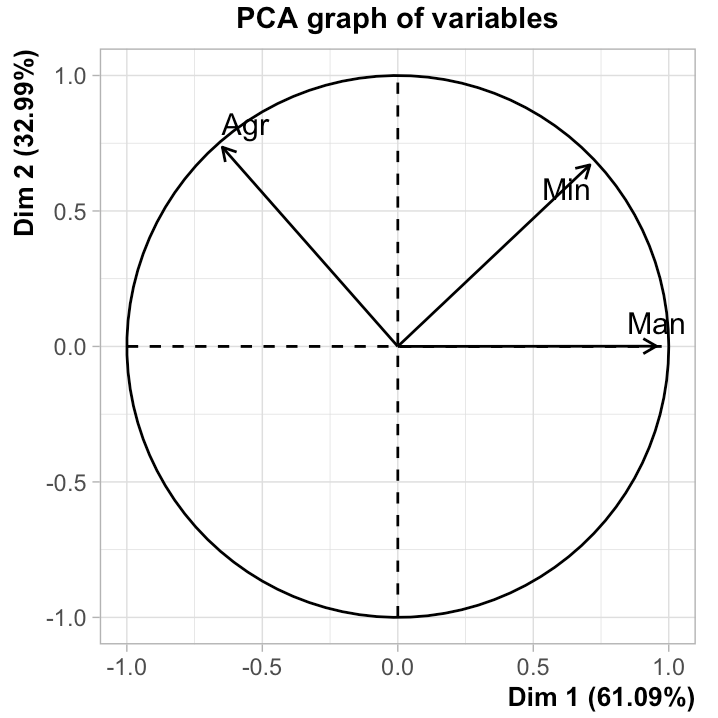
\includegraphics[scale = 0.37]{projection_variables_plan.png}
\end{figure}
    
\end{frame}

% ------------------------------------------------------------------------------------------------------------------------------

\begin{frame}[fragile]{Relations de transition}

\begin{itemize}
    \fleche On peut montrer que:
    \begin{itemize}
        \blt on peut obtenir les \motcle{composantes principales} directement par la décomposition spectrale de $\frac{1}{n}\boldsymbol{Z}\boldsymbol{Z}^\top$:
        \begin{align*}
            \boldsymbol{f}^\alpha = \boldsymbol{Z}\boldsymbol{v}_\alpha = \sqrt{\lambda_\alpha}\boldsymbol{u}_\alpha,
        \end{align*}
        \blt on peut obtenir les \motcle{vecteurs de loadings} directement par la décomposition spectrale de $\frac{1}{n}\boldsymbol{Z}^\top\boldsymbol{Z}$:
        \begin{align*}
             \boldsymbol{a}^\alpha = \boldsymbol{Z}^\top \boldsymbol{N}\boldsymbol{u}_\alpha = \sqrt{\lambda_\alpha}\boldsymbol{v}_\alpha.
        \end{align*}
        \fleche On a alors que 
        \begin{align*}
            \boldsymbol{F} &= \boldsymbol{U}\boldsymbol{\Lambda}\\
            \boldsymbol{A} &= \boldsymbol{V}\boldsymbol{\Lambda},
        \end{align*}
        où $\boldsymbol{\Lambda} = \text{diag}(\sqrt{\lambda_1}, \dots, \sqrt{\lambda_q})$.
    \end{itemize}
    \fleche En pratique, on va donc réaliser l'ACP sur un des 2 nuages (souvent le nuage des observations).
    \fleche On va ensuite dériver les résultats pour le nuage des variables sans avoir à faire la décomposition spectrale des 2 matrices.
\end{itemize}
    
\end{frame}

% ------------------------------------------------------------------------------------------------------------------------------

\begin{frame}[fragile]{Relations de transition}

\begin{itemize}
    \fleche Cela signifie que:
    \begin{itemize}
        \blt les vecteurs propres $\boldsymbol{u}_\alpha$ de $\frac{1}{n}\boldsymbol{Z}\boldsymbol{Z}^\top$ sont les \motcle{composantes principales standardisées}:
        \begin{align*}
            \boldsymbol{u}_\alpha = \frac{\boldsymbol{f}^\alpha}{\sqrt{\lambda_\alpha}},
        \end{align*}
        \blt les \motcle{loadings} sont les \motcle{corrélations entre les variables et les composantes principales}:
        \begin{align*}
            a_{j\alpha} = \text{Cor}(\boldsymbol{x}^j, \boldsymbol{f}^\alpha).
        \end{align*}
    \end{itemize}
\end{itemize}

Cette dernière propriété est importante, car elle permet de connecter la représentation des observations avec la représentation des variables. Autrement dit, elle permet de faire la représentation des observations et des variables sur le même plan. Un tel graphique est appelé \og{}biplot\fg{}.
    
\end{frame}

% ------------------------------------------------------------------------------------------------------------------------------

\section{Interprétation des résultats}

% ------------------------------------------------------------------------------------------------------------------------------

\begin{frame}{Variance des composantes principales}
    

\begin{itemize}
    \fleche Les composantes principales (colonnes de $\boldsymbol{F}$) sont \motclef{$q$ nouvelles variables} non corrélées et de variance maximale, avec
    \begin{align*}
        \text{Var}(\boldsymbol{f}^\alpha) = \lambda_\alpha.
    \end{align*}
    \fleche Il en découle que l'inertie du nuage des observations projeté sur les $q$ premières dimensions est:
    \begin{align*}
        \boldsymbol{I}(\boldsymbol{F}) = \lambda_1 + \dots + \lambda_q.
    \end{align*}
\end{itemize}

\end{frame}

% ------------------------------------------------------------------------------------------------------------------------------

\end{document}
